%% 
%% Copyright 2007, 2008, 2009 Elsevier Ltd
%% 
%% This file is part of the 'Elsarticle Bundle'.
%% ---------------------------------------------
%% 
%% It may be distributed under the conditions of the LaTeX Project Public
%% License, either version 1.2 of this license or (at your option) any
%% later version.  The latest version of this license is in
%%    http://www.latex-project.org/lppl.txt
%% and version 1.2 or later is part of all distributions of LaTeX
%% version 1999/12/01 or later.
%% 
%% The list of all files belonging to the 'Elsarticle Bundle' is
%% given in the file `manifest.txt'.
%% 

%% Template article for Elsevier's document class `elsarticle'
%% with numbered style bibliographic references
%% SP 2008/03/01

\documentclass[preprint,12pt]{elsarticle}

%% Use the option review to obtain double line spacing
%% \documentclass[authoryear,preprint,review,12pt]{elsarticle}

%% Use the options 1p,twocolumn; 3p; 3p,twocolumn; 5p; or 5p,twocolumn
%% for a journal layout:
%% \documentclass[final,1p,times]{elsarticle}
%% \documentclass[final,1p,times,twocolumn]{elsarticle}
%% \documentclass[final,3p,times]{elsarticle}
%% \documentclass[final,3p,times,twocolumn]{elsarticle}
%% \documentclass[final,5p,times]{elsarticle}
%% \documentclass[final,5p,times,twocolumn]{elsarticle}

%% For including figures, graphicx.sty has been loaded in
%% elsarticle.cls. If you prefer to use the old commands
%% please give \usepackage{epsfig}

%% The amssymb package provides various useful mathematical symbols
\usepackage{amssymb}
%% The amsthm package provides extended theorem environments
%% \usepackage{amsthm}

%% The lineno packages adds line numbers. Start line numbering with
%% \begin{linenumbers}, end it with \end{linenumbers}. Or switch it on
%% for the whole article with \linenumbers.
%% \usepackage{lineno}

\usepackage{booktabs}
\usepackage{lscape}
\usepackage{multirow}

\journal{Journal of Systems and Software}

\begin{document}

\begin{frontmatter}

%% Title, authors and addresses

%% use the tnoteref command within \title for footnotes;
%% use the tnotetext command for theassociated footnote;
%% use the fnref command within \author or \address for footnotes;
%% use the fntext command for theassociated footnote;
%% use the corref command within \author for corresponding author footnotes;
%% use the cortext command for theassociated footnote;
%% use the ead command for the email address,
%% and the form \ead[url] for the home page:
%% \title{Title\tnoteref{label1}}
%% \tnotetext[label1]{}
%% \author{Name\corref{cor1}\fnref{label2}}
%% \ead{email address}
%% \ead[url]{home page}
%% \fntext[label2]{}
%% \cortext[cor1]{}
%% \address{Address\fnref{label3}}
%% \fntext[label3]{}

\title{Variability-based improvement of m-learning applications development: product line design, implementation and experimental evaluation}

%% use optional labels to link authors explicitly to addresses:
%% \author[label1,label2]{}
%% \address[label1]{}
%% \address[label2]{}

\author[usp]{Venilton~FalvoJr}
\author[usp]{Anderson~Marcolino}
\author[usp]{Nemesio~Duarte~Filho}
\author[uem]{Edson~OliveiraJr}
\author[usp]{Ellen~Barbosa\fnref{myfootnote}}

\fntext[myfootnote]{Institute of Science and Computational Mathematics (ICMC-USP), Avenida Trabalhador Sao-Carlense, 400, Sao Paulo, Brazil. E-mail: francine@icmc.usp.br. Phone: +55 (16) 3373-8177. Fax: +55 (16) 3373-8888.}

\address[usp]{University of Sao Paulo (USP), Brazil}
\address[uem]{State University of Maringa (UEM), Brazil}

\begin{abstract}
Software Product Lines (SPL) aim at improving the product quality and time-to-market of singular software development methodology. This reuse approach has variability as a central concept that allows the diversity of software products in a specific domain. On the educational domain, the popularity of mobile devices has contributed to the increasing demand for mobile learning (m-learning) applications. This paper discusses how variability can improve the development of m-learning applications by adopting SMarty a concise variability management approach. An SPL for m-learning applications was developed and experimentally evaluated industry, providing evidence that well-defined variabilities can speed up time-to-market of m-learning products with reduced number of faults.
\end{abstract}

\begin{keyword}
software product lines \sep mobile learning \sep variability management \sep experimental evaluation
%% keywords here, in the form: keyword \sep keyword

%% PACS codes here, in the form: \PACS code \sep code

%% MSC codes here, in the form: \MSC code \sep code
%% or \MSC[2008] code \sep code (2000 is the default)

\end{keyword}

\end{frontmatter}

%% \linenumbers

%% main text
\section{Introduction}

Constantly changes in software reuse approaches lead to the concept of Software Product Line (SPL), which represents a shift in focus from the singular software development paradigm. From this concept, companies that previously developed project-by-project software have now focused on the creation and maintenance of SPL and their variabilities. Thus, models that represent variabilities are specified as part of the core assets of an SPL, in which their correct identification, specification and representation allow to take several development benefits \cite{chen11, capilla13}.

To manage the variabilities that allow to diversify the portfolio of products in a given domain, it is necessary the adoption of a well-defined systematic approach. Some of these approaches may be used in Domain Engineering (DE) and Application Engineering (AE), supporting the selection and delimitation of the variant artifacts from different products \cite{bockle05, vanderlinden07}.

For an SPL to be successful, its domain must be defined carefully. If the domain is too large and product members vary too widely, the core assets will be strained beyond their ability to accommodate the variation, economies of production will be lost, and the product line will collapse into an old-style, one-at-a-time product development effort. If the domain is too small, the core assets might not be built in a generic enough fashion to accommodate future growth, and the product line will stagnate: economies of domain will never be realized, and the full potential return on investment (ROI) will never materialize \cite{bockle05, vanderlinden07}.

In a different but related perspective, the rapid growth of information and communications technologies has favored the emergence of innovative ways to face the shortcomings of traditional education \cite{west12}. In this context, mobile learning (m-learning) has emerged, providing a strong interaction between learners and instructors, enabling them to actively participate of the knowledge construction process anytime and anywhere \cite{kukulska05}. 

M-learning has grown in terms of importance and visibility, mainly because of significant results with regard to flexibility and propagation of education \cite{kinshuk03, wexler08}. These aspects have made of m-learning a promising tool on behalf of education. In 2011, the first ``UNESCO Mobile Learning Week'' suggested m-learning as an alternative to that which UNESCO called ``teacher crisis'', expression justified by global need for 8.2 million new teachers to achieve the UN Millennium Development Goal of providing universal primary education by 2015 \cite{west12}.

Due to the diversity of platforms, technologies and pedagogical methods that can be considered for the development of m-learning applications, a wide range of specificities  may be streamlined and addressed through a reuse perspective. However, there are few works addressing development issues through a strategy of systematic reuse, such as SPL, for mobile middleware and, consequently, for the m-learning domain as well \cite{bezerra09}.

Motivated by this scenario, we have worked on the establishment of M-SPLearning, an SPL to the m-learning domain~\cite{falvojr14a, falvojr14b}. M-SPLearning has been developed based on a concise UML-based variability management approach, named SMarty~\cite{oliveirajr10}, which provides mechanisms to facilitate the identification and representation of variabilities.

This paper discusses how variability improves the development of m-learning applications by means of the use of SMarty. We experimentally evaluated M-SPLearning with respect to singular software development, particularly comparing time-to-market and quality of the software products implemented from the use of both (SPL and singular) approaches. The results showed a significant reduction of time-to-market and a quality improvement, in terms of faults, when considering the software products developed from the M-SPLearning core assets with the support of variabilities.

The paper is organised as follows.  Background is summarized in Section \ref{section2}, M-SPLearning is described in Section \ref{section3}. In Section \ref{section4}, we present the experimental evaluation performed. In Section \ref{section5} we discuss the lessons learned from the development and application of M-SPLearning. Related work is presented in Section \ref{section6}. Conclusions and perspectives for future work are discussed in Section \ref{section7}.

\section{Background}\label{section2}

In this section we provide a brief overview of essential concepts with respect to: (i) SPLs and variabilities; (ii) the SMarty approach for variability management; and (iii) m-learning.

\subsection{SPL and Variabilities}

SPLs enable the creation of software-intensive systems that share and manage a set of features satisfying the specific needs of a particular domain. Commonalities are shared by all derived products, while variabilities represent the scope of customization supported by them \cite{bockle05,vanderlinden07}.

%The proper management of variabilities has great relevance in order to ensure that all the benefits of SPLs are obtained. In this sense, different approaches related to the management of variabilities have been discussed by the research community.

Variability is one of the most important issues in designing an SPL, reflecting the way according to which family members of an SPL differ from each other. The precise and explicit representation and management of variabilities make possible the consistent generation of specific products in an SPL \cite{chen11, capilla13}. 

Variabilities can be initially identified and represented by means of features, which represent relevant and visible characteristics to stakeholders of a particular domain \cite{bosch01}. Features are usually represented by a feature model, i.e., a hierarchical representation that captures the structural relationships among the features of a specific domain \cite{bockle05, vanderlinden07}. Common features to the SPL products are considered mandatory, while variable features can be optional or alternative. %To be included in a product, optional features should add some value to its mandatory features. Two or more features may be alternative, however, only one may be included in a particular product.

The concept of SPL is suitable to domains in which there is a demand for products that have common features and a well-defined set of variabilities. For instance, considering the education domain, instructors, tutors and apprentices can use ubiquitous computing to contribute and access the learning materials anytime and anywhere \cite{kukulska05}. This characteristic is achieved due to variabilities, such as interactivity and multimedia resources \cite{falvojr14a, falvojr14b}, which provide a high degree of communication and cooperation among users.

At its essence, the conception of an SPL involves core asset development and product development, both under a technical and organizational management perspectives. Core asset development can be done with extraction of artifacts from existing software products or through scratch development and, with the existent artifacts, the products can be development. Generally, products and core assets are built in common according among them. These SPL's conception phases are classified into three essential activities: (i) Core Asset Development or DE; (ii) Product Development or AE; and (iii) Management \cite{bockle05, vanderlinden07}.

\subsection{The SMarty Approach}

The proper management of variabilities has great relevance to ensure that all the benefits of SPLs are obtained. Different approaches related to the management of variabilities have been proposed by the research community  \cite{chen11, capilla13}.  

%The choice of an approach that supports the representation of technical models is a difficult task due to the wide range of existing proposals and, at the same time, the lack of experimental validation of them. While some of the existing approaches use specific domain languages, others are based on widely known modeling languages, such as UML.

%M-SPLearning has been developed based on a variability management approach -- SMarty (\textbf{S}tereotype-based \textbf{M}anagement of V\textbf{ar}iabili\textbf{ty}) approach~\cite{junior2010, fiori2012}. Among the reasons for our choice, we highlight: (i) the cognitive ease provided by SMarty, supporting the adoption of modeling tools; (ii) its conformance with UML, facilitating the development and validation of SPLs; and (iii) the existence of experimental evidences with regard to its use~\cite{marcolino2013, marcolinocls2014, marcolinoseq2014}. 

\textbf{S}tereotype-based \textbf{M}anagement of V\textbf{ar}iabili\textbf{ty} (SMarty)~\cite{oliveirajr10} is a variability management approach, composed of an UML 2.4 profile, the SMartyProfile, and supported by a systematic process, the SMartyProcess, related to the main SPL activities. The SMartyProcess defines a set of guidelines, which supports the application of stereotypes and tagged-values from the SMartyProfile. The guidelines ensure the identification and representation of variabilities and allow the evolution of SPL, whereas the process incrementally and iteratively guarantees the identification of new variabilities and the evolution of the SPL core assets.

Another benefit from the use of SMarty is the visibility with respect to the relationship among the feature model and the variabilities in the UML diagrams. The variabilities composed of variation points are fully represented, eliminating the need of additional documents to perform the development \cite{oliveirajr10}.

%\footnote{A variation point specifies the points where the variation occurs and may be solved by choosing one or more variants, ruled by a set of constraints \cite{pohl2005}.}

The UML models supported by SMarty (use case, class, sequence, component and activity) represent the static and dynamic aspects of software products.  In recent studies, the SMarty effectiveness with respect to identification and representation of variabilities in the UML models was experimentally evaluated \cite{marcolino13, marcolino14a, marcolino14b, bera15}. The results provided evidence of the effectiveness from use case, sequence and component models. Also, they lead to the evolution of the SMartyProcess for class models.

%The identification of some issues and the solution of them in new versions allows a better precision and confiability in the utilization and adoption of the approach. Beside this facts, the SMartyProcess allows a quickly learning process of their profile and its application for the software product line developed.


%The guideline below exemplifies how its use facilitates the application and evolution of a SPL. The guideline is identified by an acronym and a number. This example shows the second (2) guideline for use case diagram (UC) \footnote{Detailed descriptions of the guidelines are in \cite{junior2010, fiori2012}}.

%\textbf{UC.2} elements of use case models related to the include (dependency - $<<$include$>>$) or association from actors relationships suggest either mandatory or optional variants.

%Moreover, the set of guidelines facilitates the analysis of the UML semantic elements, associating them to the variable elements of an SPL. This helps on the identification of new variabilities, and supports the development process by the product line engineer.

%The complexity and amount of variabilities and similarities to be managed in a SPL, if kept by a concise approach, allows a quickly generation of consistent products, as demonstrated by the experimental study presented in this paper (Section \ref{sec:exp}).

\subsection{Mobile Learning}

%The education and knowledge seeking represent an increasingly a necessity for anyone who wants to be competitive and successful, regardless of their age, gender or ethnicity. This scenario, coupled with 

The rapid growth of information and communication technologies has favored the emergence of new methods for teaching and learning, providing innovative ways to face the shortcomings of traditional education \cite{west12}. 

M-learning has emerged in this context, being characterized by the ability to provide a strong interaction between learners and instructors, enabling them not only to access a virtual learning environment but also to contribute and actively participate of the knowledge construction process through mobile devices anytime and anywhere \cite{kukulska05}. Thus, the interaction with learning applications through mobile devices provides benefits that go beyond accessibility, convenience and communication.

%(e.g., mobile phones, tablets, smartphones, laptops, tv, etc.)  

%In this context, issues related to teaching and learning have been increasingly discussed and studied by the scientific community. In particular, computational learning environments are showing a increasing importance, performing a vital role in teaching and training activities, being relevant not only in the academic field but also in the industrial environment \cite{svetlana2009}.

%If we consider the characteristics of the current society in a parallel with their latest technological evolutions, perhaps the most effective method of teaching is the mobile apredizado, or simply m-learning \cite{unesco2012}. In general, m-learning is characterized by the ability to provide a strong interaction between learners and instructors, enabling them to contribute, participate and access the learning environment through mobile devices (phones, tablets, smartphones, laptops, tv, etc.) anytime and anywhere \cite{kukulska2005}.

Despite the benefits provided, m-learning is still considered an incipient concept, presenting limitations that difficults its effective development and adoption. For instance, even with the increasing demand for m-learning applications, there are few works addressing development issues through a strategy of systematic reuse, such as SPL, in the mobile learning setting.  

Based on the concepts and ideas summarized in this section, we have worked on the establishment of M-SPLearning, an SPL to the m-learning domain. The main characteristics of M-SPLearning as well as its evaluation by conducting an experimental study are discussed next. 

%Being a relatively new concept and that gained momentum with its current ubiquity, the m-learning represents an attractive line of research due to the lack of methodologies that potentialize him. In this sense, the many settings and tools existing in the applications of this area provide a favorable scenario for implementing a strategy of systematic reuse. Consequently, the authors explore this niche through M-SPLearning, which synthesizes an LPS applied to the field of m-learning applications \cite{seke2014, fie2014}.

\section{M-SPLearning}\label{section3}

%Com o objetivo de apresentar como o gerenciamento da variabilidades pode melhorar o desenvolvimento de aplicações de m-learning, os autores definiram uma LPS, denominada M-SPLearning. Buscando explorar as variabilidades desse domínio para acelerar o time to market e reduzir o numero de falhas nos produtos. Nesta seção, as atividades conduzidas para a concepção da M-SPLearning são detalhadas a fim de expor suas principais peculiaridades e referências.
Aiming at presenting how the management of variabilities can improve the development of m-learning applications, we have established M-SPLearning \cite{falvojr14a, falvojr14b}. The idea is to investigate how the variabilities of this domain can accelerate time-to-market and reduce product faults. In this section, the activities conducted in design of the M-SPLearning are detailed \cite{oliveirajr10, filho13, krueger02, kang90}.

%A Seção \ref{section31} apresenta a Engenharia de Domínio realizada para concepção da \textit{M-SPLear\allowbreak ning} evidenciando sua capacidade produtiva através das seguintes atividades secundárias: (i) Análise de Domínio; (ii) Definição da Arquitetura; (iii) Projeto de Componentes; e (iv) Plano de Produção. Em seguida, na Seção \ref{section32}, a Engenharia de Aplicação apresenta os detalhes sobre a implementação e utilização da LPS especificada.
%Section \ref{section31} presents the DE performed for the M-SPLearning design showing its productive capacity by means of the following sideline activities: (i) Domain Analysis; (ii) Definition of Architecture; (iii) Components Design; and (iv) Production Plan. In Section \ref{section32}, AE details the implementation and utilization of our SPL.

\subsection{Domain Engineering}\label{section31}

%Durante a atividade de Engenharia Domínio as similaridades e variabilidades devem ser eliciadas para o desenvolvimento de LPS, a fim de estabelecer uma plataforma reutilizável sistemática. O resultado desta atividade é um conjunto de ativos com os quais a LPS deve ser implementada, caracterizando, assim, sua família de produtos. Em geral, as actividades que caracterizam a Engenharia de Domínio pode ser consideradas as mais críticas durante a concepção de uma LPS, dado que delimitar um domínio de estudo não é uma tarefa trivial.
During the DE activity, similarities and variabilities must be specified for the development of the SPL in order to establish a systematic reusable platform. The result of this activity is a set of assets from which the SPL should be implemented, thus characterizing its product family \cite{bockle05, vanderlinden07}. In general, the activities that characterize the DE can be considered the most critical in the conception of an SPL, since delimiting a domain of study is not a trivial task.

%Analisando o extenso domínio das aplicações móveis percebe-se que seus produtos podem ser implementadas usando diferentes plataformas de desenvolvimento, como por exemplo, Android, iOS ou Windows Phone. Com isto, o domínio de m-learning também inclui sistemas operacionais diferentes. Assim, para definir um domínio aceitável em termos de escopo, selecionamos um único sistema operacional. Nossa escolha pelo Android se baseou na quantidade de dispositivos que cada sistema operacional controla, visto que esse SO detém cerca de 80% do mercado de smartphones do mundo, equivalente a 793,6 milhões de dispositivos.
Mobile applications can be implemented using different development platforms, including Android, iOS and Windows Phone. Furthermore, the m-learning domain also includes different operating systems. Thus, to define an acceptable domain in terms of scope, we selected a single operating system. Our choice for Android was based on the amount of devices that each operating system controls, since this OS owns around 80\% of the world's smartphones market, which is equivalent to 793.6 million devices. \cite{llamas14}.

%Com um domínio factível definido, um catálogo de requisitos para ambientes m-learning foi adaptado respeitando o modelo de qualidade ISO/IEC 25010, gerando, assim, um catálogo de requisitos estendido e, em seguida, o modelo de features para a M-SPLearning. Tal catálogo busca refletir, em alto nível, a experiência adquirida pelos desenvolvedores e pesquisadores nesta nova modalidade de aprendizagem. Além disso, o catálogo é genérico e abrangente, beneficiando sua adoção para fins diferentes do domínio de m-learning.
With a feasible domain defined, a requirements catalog for m-learning applications was proposed based on a related work \cite{filho13} and ISO/IEC 25010 quality model. Such a catalog intends to reflect, in a high level basis, the experience gained from developers and researchers of m-learning. Furthermore, the catalog is generic and embracing, benefiting its adoption for different purposes in the m-learning domain. 

%Para o gerenciamento das variabilidades em questão a M-SPLearning foi desenvolvida com base na abordagem SMarty. Entre as razões para a nossa escolha, destacam-se: (i) a facilidade cognitiva fornecida pela SMarty, apoiada por várias ferramentas de modelagem; (ii) a sua conformidade com UML, facilitando o desenvolvimento e validação da SPLs; e (iii) a existência de evidências experimentais no que diz respeito à sua utilização.
For the management of variabilities in question, the M-SPLearning has been developed based on the SMarty approach~\cite{oliveirajr10}. Among the reasons for our choice, we highlight: (i) the cognitive ease provided by SMarty, supported by several modeling tools; (ii) its compliance with UML, which facilitates the development and validation of SPLs; and (iii) the existence of experimental evidence with regard to its use~\cite{marcolino13, marcolino14a, marcolino14b, bera15}. 

%Em termos práticos, as atividades para a implementação de uma LPS não são triviais e exigem tempo e esforço consideráveis, o que compromete a sua aceitação na indústria. Com o objetivo de reduzir as barreiras de adoção desse conceito foram consideradas três estratégias: proativo, reativo e extractivo.
In practical terms, the activities for implementing an SPL are not trivial and require considerable time and effort, which undermines their acceptance in industry. Aiming to define an appropriate adoption strategy to the concept of SPL, the proactive, reactive and extractive models can be considered.
%Tais modelos foram analisados considerando o contexto deste trabalho, assim a abordagem proativa foi escolhida. Essa estratégia é plenamente aplicável ao contexto da M-SPLearning, uma vez que é apropriada quando os requisitos para o conjunto de produtos a serem desenvolvidos são estáveis e podem ser previamente definidos, condição fornecida pelo catálogo de requisitos relacionado à LPS.
Each model was analyzed considering the context of this work, and the proactive approach was chosen. This strategy is fully applicable to the context of M-SPLearning, since it is the most appropriate when the requirements for the set of products to be developed are stable and can be previously defined. This condition was satisfied by the proposed requirements catalog.

%A partir desse conjunto de definições, foram conduzidas quatro atividades no escopo da Engenharia de Domínio. Seus respectivos papeis e saídas são descritos nas subseções a seguir.
%Based on this set of definitions, four activities were conducted within the scope of DE. Their respective roles and outputs are described in the following subsections.

\subsubsection{Domain Analysis}\label{domainAnalysis}

%De acordo com o modelo de adoção proativo proposto por \citet{krueger2001}, primeiramente é realizada a Análise de Domínio e escopo, com o propósito de identificar a variação dos produtos apoiados pela LPS. Para isso, o catálogo de requisitos proposto por \citet{filho2013} foi confrontado com o modelo de qualidade ISO/IEC 25010 \cite{iso2011}, com o objetivo de identificar requisitos de qualidade ausentes ou desconexos em termos negociais e hierárquicos.
According to the proactive model, the domain and scope analysis should be is performed primarily, in order to explore the variation of the products supported by an SPL \cite{krueger02}. To do so, the requirements catalog \cite{filho13} was analysed with respect to the quality model ISO/IEC 25010, in an attempt identify missing or disconnected quality requirements.
%A partir dessa análise alguns requisitos foram reagrupados, renomeados e, em menor proporção, adicionados e removidos do catálogo de requisitos. Essas modificações consideraram o escopo e domínio definidos para a M-SPLearning, gerando assim uma derivação do catálogo original, ilustrado na Figura \ref{fig:msplCatalogo}.
From this analysis some requirements have been regrouped, renamed and, in few cases, added and removed from the requirements catalog. The final requirements catalog is illustrated in Figure \ref{figureMSPLCatalog}.

\begin{figure}
    \centering
    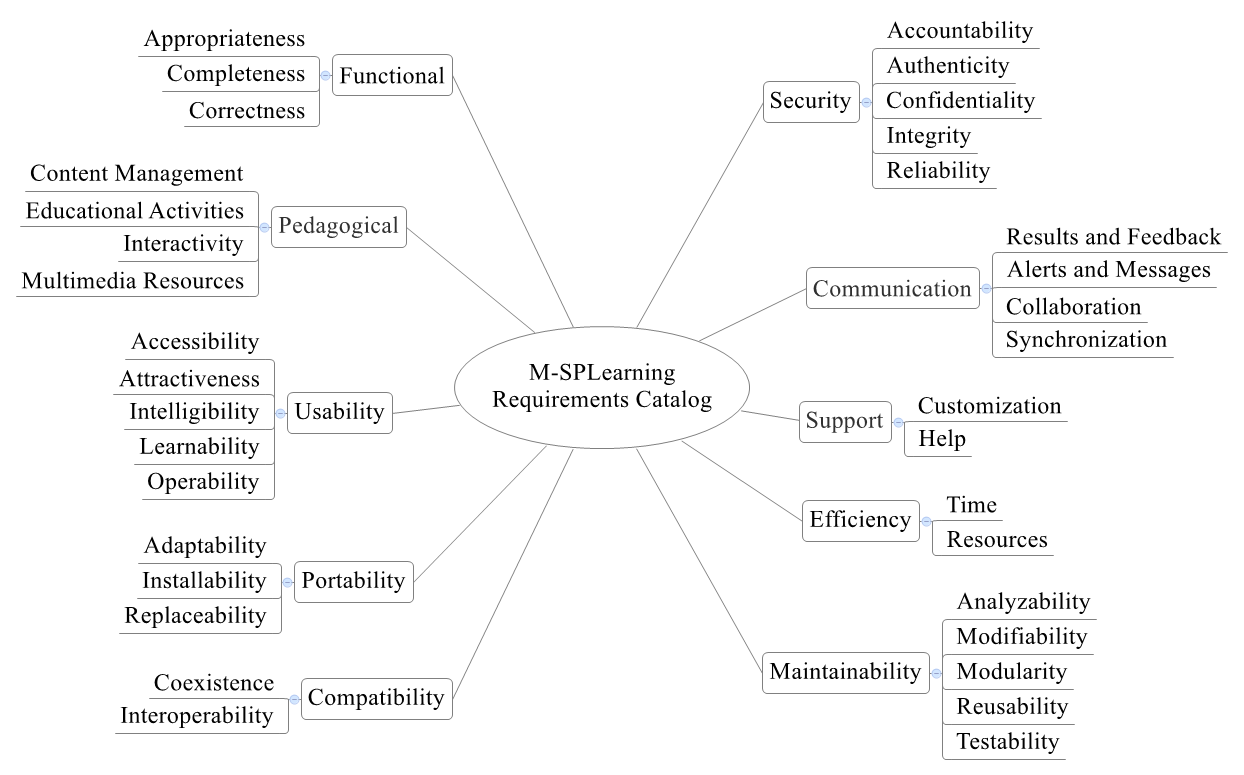
\includegraphics[scale=0.3815]{figures/section3/MSPLCatalog}
    \caption{M-SPLearning Requirements Catalog \cite{falvojr14b}.}
    \label{figureMSPLCatalog}
\end{figure}

%Com base no catálogo de referencia, observou-se que a maioria dos requisitos originalmente propostos eram equivalentes, direta ou indiretamente, às características e subcaracterísticas da norma ISO/IEC 25010. Com isso, acredita-se que a derivação do catálogo forneceu os requisitos educacionais móveis necessários para a concepção da LPS deste trabalho.
Based on the reference catalog, we could observe that most of the requirements originally proposed was equivalent, directly or indirectly, to the characteristics and subcharacteristics of ISO/IEC 25010. %Thus, it is believed that the performed  derivation provided us the educational requirements necessary for the M-SPLearning.
%Em termos estruturais, o catálogo resultante apresentou 10 requisitos primários e 35 secundários. Por exemplo, o elemento Support apresenta características comuns como a internacionalização de mensagens (provida pelo requisito Customization) e ajuda em dúvidas frequentes (Help).
In structural terms, the resulting catalog has 10 primary and 35 secondary requirements. For example, the \textit{Support} element has common features such as internationalization of messages (provided by \textit{Customization} requirement) and helps to frequently asked questions (\textit{Help}).

%Apesar de possuir requisitos genéricos e aplicáveis a outros domínios, o catálogo proposto também possui características específicas para aplicações m-learning. Por exemplo, a maior parte dos requisitos derivados a partir de Pedagogical e Communication representam necessidades essenciais ao domínio educacional móvel.
Despite having generic requirements, the proposed catalog also has specific features for m-learning applications. For instance, most of the requirements derived from \textit{Pedagogical} and \textit{Communication} represent essential requirements to the mobile educational domain.

%Em termos pedagógicos, o gerenciamento de conteúdos educativos é fundamental para o desenvolvimento das atividades educacionais. Além disso, a presença de recursos multimédia pode proporcionar acesso a informação de uma forma mais atrativa. Tais peculiaridades sintetizam os requisitos classificados pelo item Pedagogical.
In pedagogical terms, the educational content management is essential for the development of educational activities. Furthermore, the presence of multimedia resources can provide access to information in a more attractive way. Such peculiarities summarize the requirements classified by the \textit{Pedagogical} item.

%Por sua vez, os requisitos provenientes de Comunucation representam funcionalidades relacionadas à troca de mensagens, alertas e o compartilhamento de resultados ou feedbacks, tornando o aprendizado, mais colaborativo e dinâmico. Outra característica importante é a sincronização dos dados de uma aplicação m-learning, pois os usuários podem possuir e utilizar mais de um dispositivo móvel ou plataforma. 
The requirements from \textit{Communication}, in turn, represent features related to the exchange of messages, alerts and sharing results or feedback, making the learning more collaborative and dynamic. Another important feature is the synchronization of data from a mobile learning application since users can have more than one mobile device or platform.

%A fim de avaliar o catálogo de requisitos proposto para a M-SPLearning uma validação adicional actividade foi conduzida. Neste sentido, um formulário on-line foi preparado a fim de verificar informalmente as principais questões técnicas relacionadas ao catálogo. O formulário foi disponibilizado em uma estrutura de checklist, com o objetivo de mensurar a opinião de especialistas na área de engenharia de software.
To evaluate the requirements catalog proposed for the M-SPLearning, an additional validation activity was conducted. An online form was prepared in order to informally check the main technical issues related to the catalog. The form was structured as a checklist, with the aim to measure the opinions of specialists in software engineering area.

%O documento contou com 12 questões de múltipla escolha, onde as duas primeiras eram relacionadas à experiência dos participantes nos conceitos de LPS e m-learning. Nesse caso, as opções possíveis foram: Proficiente, Intermediário e Novato. As dez  questões restantes referiam-se ao catálogo de requisitos da M-SPLearning, por exemplo: O catálogo compreende requisitos adequados ao domínio?. Para essas perguntas as opções: Adequado, Regular e Insatisfatório foram aplicadas.
The checklist was composed of 12 multiple choice questions, where the first two questions were related to the background of the participants on SPL and m-learning concepts. In this case, the possible options were ``Expert", ``Intermediate" and ``Novice". The ten remaining questions were related to the M-SPLearning requirements catalog, such as: \textit{``The catalog comprises appropriate requirements to the domain?"}. To these questions the options ``Adequate", ``Regular" and ``Unsatisfactory" were applied.

%Para aplicação do formulário online alguns grupos de pesquisa foram notificados via e-mail com um convite para a participação voluntária no checklist. Após alguns dias o formulário foi finalizado com um total de 11 participantes.
%To apply the online form several research groups were notified via email with an invitation for voluntary participation in the checklist. After a few days the form was completed with a total of eleven participants.

%Os resultados coletados mostraram que, na visão dos participantes, o catálogo de requisitos está adequado ou regular a todos os itens avaliados. Além disso, nenhuma das questões relacionadas ao catálogo de requisitos da M-SPLearning foi respondida como insatisfatória. A Tabela \ref{tableMSPLChecklist} sintetiza as avaliações médias obtidas a partir dos 11 formulários de ckecklist submetidos.
The questionnaire was answered by 11 participants and the results showed that the requirements catalog was ``Adequate", with a mean of 60.90\%, and was ``Regular", with a mean of 39.10\%, in all evaluated items. Furthermore, none of the questions related to the requirements catalog of the M-SPLearning was answered as ``Unsatisfactory". 

%Table \ref{tableMSPLChecklist} summarizes the average ratings obtained from submitted forms.
%
%\begin{table}
%    \caption{M-SPLearning Requirements Catalog Checklist Summary.}
%    \centering
%    \scriptsize
%    \begin{tabular}{cc}
%        \toprule
%        \textbf{Option} & \textbf{Average Percentage Obtained} \\
%        \midrule
%        Adequate       & 60.90\% \\
%        Regular        & 39.10\% \\
%        Unsatisfactory & 0.00\% \\
%        \bottomrule
%    \end{tabular}
%    \label{tableMSPLChecklist}
%\end{table}
%
%A sumarização dos resultados foi considerada uma validação preliminar, visto que o preenchimento de um checklist anônimo não caracteriza uma técnica de validação formal. Desta forma, o checklist proposto consistiu em uma validação inicial que deve ser complementada com novas técnicas no futuro. Todavia, esta atividade de validação foi importante para avaliar o artefato que sintetizou os requisitos elicitados para a M-SPLearning.
%The summary of the results was considered a preliminary validation, since the completion of an anonymous checklist does not characterize a formal validation technique. Therefore, the proposed checklist consisted of an initial validation that should be supplemented with new techniques in the future. However, this validation activity was important to evaluate the asset that summarized the elicited requirements for the M-SPLearning.
Although preliminary, the informal validation performed was important to evaluate the set of requirements elicited for M-SPLearning.

%A próxima etapa da atividade de Análise de Domínio consiste em identificar as variabilidades existentes nos produtos da M-SPLearning, de acordo com a definição da abordagem proativa. Nesse sentido, as variabilidades representam a forma pela qual os produtos são diferenciados em uma LPS, tornando possível a geração dos produtos específicos suportados pela LPS. Em termos práticos, as variabilidades geralmente são identificadas e representadas através do conceito de features.
The next stage of the Domain Analysis activity was the identification of the existing variabilities in the M-SPLearning products \cite{krueger02}. In this sense, variabilities represent the way in which products are differentiated in an SPL, making possible the generation of specific products supported by the SPL \cite{vangurp01}. In practical terms, variabilities are generally identified and represented through the features concept \cite{bosch01, kang90}.

%No contexto da M-SPLearning, o catálogo de requisitos foi analisado, e suas características serviram como base para a criação de um modelo feature em conformidade aos requisitos elicitados (Figura X). A interpretação do modelo de features é simples e segue os conceitos tradicionais idealizados pela abordagem Feature-Oriented Domain Analysis (FODA). Basicamente, cada requisito concreto presente no catálogo M-SPLearning foi transformado em uma feature primária. Com isso, foram modeladas 16 features obrigatórias e 14 features opcionais.
In the context of M-SPLearning, the requirements catalog was analyzed and their characteristics were used as the basis for creating a feature model with compliance to the requirements elicited (Figure \ref{figureMSPLFeatureModel}). The interpretation of the feature model is straightforward and follows the traditional concepts conceived by the Feature-Oriented Domain Analysis approach (FODA) \cite{kang90}. Basically, each concrete requirement in M-SPLearning catalog was mapped to a primary feature. Thus, 16 mandatory features and 14 optional features were modeled.



%Com relação ao catálogo, alguns dos requisitos elicitados foram considerados muito abstratos ou onipresentes em relação do domínio m-learning e, por isso, não foram transformados em features, são eles: (i) Functional; (ii) Portability; (iii) Efficiency; e (iv) Maintainability. Por outro lado, as features primárias e suas respectivas responsabilidades no domínio das aplicações m-learning são apresentadas a seguir, sintetizando as contribuições relacionadas à Análise de Domínio:
With regard to the catalog, some of the elicited requirements were considered too abstract or ubiquitous over the m-learning domain and, therefore, they were not mapped to features (\textit{Functional}, \textit{Portability}, \textit{Efficiency}, \textit{Maintainability}). The primary features and their responsibilities for m-learning applications are the following:

\begin{itemize}

    %Incorpora requisitos educacionais e pedagógicos, provendo as principais características presentes em aplicações m-learning para atividades de ensino e treinamento. A subfeature Interactivity é opcional, uma vez que está relacionada a interatividade por meio de redes sociais. As subfeatures Content Management, Educational Activities e Multimedia Resources são obrigatórias, onde a última delas possibilita a escolha de um ou mais recursos multimédia como apoio ao ensino.
    \item \textit{Pedagogical}: incorporates educational and pedagogical requirements, providing the main characteristics of m-learning applications for teaching and training activities. The subfeature \textit{Interactivity} is optional, as it is related to interactivity through social networks. The subfeatures \textit{Content Management}, \textit{Educational Activities} and \textit{Multimedia Resources} are mandatories; in the latter offers a choice of one or more multimedia resources to support teaching.
    
    %Apresenta características essenciais no que diz respeito à interface visual de uma aplicação m-learning. Tais características são fundamentais para a aceitação do produto no mercado. Essa feature e suas variações determinam que todos os produtos gerados pela LPS devem ter um padrão de usabilidade, provendo qualidade aos usuários finais. Com isso, todas as features em questão foram definidas como obrigatórias.
    %A plataforma Android possui diversas imposições em termos de usabilidade, com o objetivo de padronizar e maximizar a experiência de seus usuários, por este motivo as features em questão foram definidas como abstratas.
    \item \textit{Usability}: address the essential characteristics with respect to the visual interface of a mobile learning application. These characteristics are fundamental to the acceptance of the product on the market. This feature and its variations establish that all products generated by an SPL must adopt a standard of usability, providing quality to final users. Thus, all these features were defined as mandatory.


\begin{figure}[!ht]
    \centering
    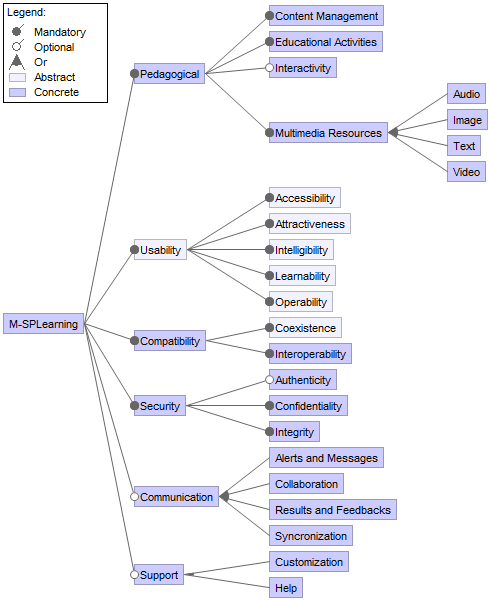
\includegraphics[scale=0.8]{figures/section3/MSPLFeatureModel}
    \caption{M-SPLearning Feature Model \cite{falvojr14a, falvojr14b}.}
    \label{figureMSPLFeatureModel}
\end{figure}

    %Engloba a coexistência e capacidade de trocar informações com outros sistemas no mesmo ambiente operacional. Por se mostrar essencial a aplicativos móveis, essas features foram definidas como obrigatórias.
    \item \textit{Compatibility}: includes the coexistence and ability to exchange information with other systems on the same operating environment. It is essential for mobile applications, thus their features were defined as mandatory.
    
    %Trata-se de uma feature fundamental para qualquer aplicativo m-learning, uma vez que existem aspectos que devem ser garantidos para que os usuários confiem no produto gerado. As features que representam a integridade e confidencialidade foram definidas como obrigatórias devido a sua importância em termos de seguraça. Já a feature Authenticity é opcional porque nem todo aplicativo m-learning possui autenticação explícita de seus usuários.
    \item \textit{Security}: this is a key feature since any mobile application should send and receive data securely. The features \textit{Integrity} and \textit{Confidentiality} were defined as mandatory due to its importance in security terms. On the other hand, the \textit{Authenticity} feature is optional because not every m-learning application has explicit authentication of its users.
    
    %Provê o transporte de informações entre os usuários do aplicativo, possibilitando a troca de mensagens, a verificação resultados de testes e até mesmo a sincronização de atividades realizadas em outros dispositivos móveis. Essa feature é opcional e suas subfetaures possuem essa mesma definição, possibilitando qualquer combinação possível entre elas.
    \item \textit{Communication}: responsible for changing information among users of the application, enabling the exchanging of messages, testing results and even synchronizing activities in other mobile devices. This feature and subfeatures are optional, allowing any possible combination among them.
    
    %Trata-se de uma feature considerada um diferencial de qualidade para os produtos em que ela está presente, pois provê alternativas de apoio ao usuário, como ajuda e internacionalização. Foi classificada como opcional por não ser um pré-requisito, assim como suas subfeatures.
    \item \textit{Support}: this feature provides some interesting alternatives to user, such as help and internationalization. It was classified as an optional because it is not a prerequisite as well as its subfeatures.
\end{itemize}

\subsubsection{Definition of Architecture}

%A partir do modelo de features apresentado anteriormente, definimos uma arquitetura de software aderente às necessidades do domínio educacional móvel. Tal arquitetura e seus respectivos componentes representam de forma abstrata os ativos centrais da M-SPLearning. Nesse sentido, a maioria das abordagens desenvolvidas para auxiliar no gerenciamento de variabilidades envolvem diversos conceitos e modelos de representação. A abordagem SMarty, em especial, é baseada na UML, amplamente aceita pela comunidade científica. Com isso, devido a sua facilidade de uso e resultados experimentalmente avaliados a SMarty foi escolhida para apoiar esta atividade da M-SPLearning.
From the feature model we defines an adherent software architecture to the mobile domain educational needs. Such an architecture and its components represent abstractly the core assets of M-SPLearning. Accordingly, most of the approaches developed to assist in the management of variability involve several concepts and representation models. SMarty, in particular, is based on UML, widely accepted by scientific and industrial communities. Thus, due to its ease of use and results (experimentally evaluated), SMarty was chosen to support the design of the M-SPLearning promising architecture.

%A abordagem SMarty foi essencial durante todo o processo de desenvolvimento da LPS proposta, sobretudo por agregar seu perfil aos modelos UML para representação das similaridades e, principalmente, das variabilidades da M-SPLearning, como é o caso do diagrama de componentes arquiteturais ilustrado na Figura \ref{figureMSPLArchitecture}. Com base no diagrama arquitetural é possível identificar a base estrutural utilizada para a construção da M-SPLearning. O pacote com os ativos centrais engloba os componentes que representam as features definidas como concretas no modelo de features.
SMarty played a important role through the development of M-SPLearning, providing the standards defined by the SMartyProfile to represent the similarities and, especially, the variabilities of M-SPLearning. The diagram of architectural components illustrated in Figure \ref{figureMSPLArchitecture} represents one of the diagrams developed with the support of the SMarty approach. Based on the architectural diagram it is possible to identify the structural basis used to the construction of the M-SPLearning. The package \textit{Core Assets} comprises concrete features as shown on Figure \ref{figureMSPLFeatureModel}.

\begin{figure}
    \centering
    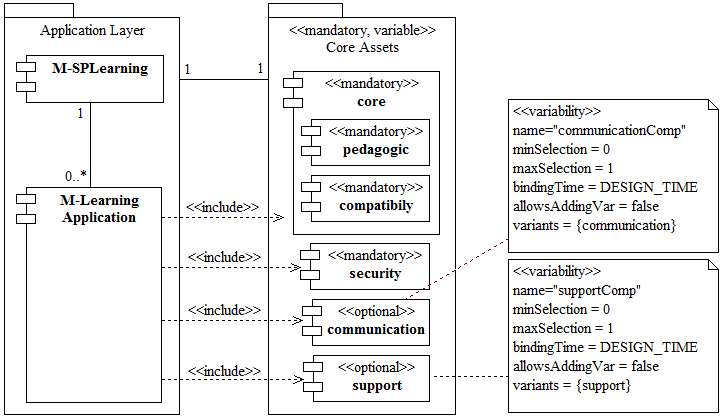
\includegraphics[scale=0.55]{figures/section3/MSPLArchitecture}
    \caption{M-SPLearning SMarty-based Architecture Diagram.}
    \label{figureMSPLArchitecture}
\end{figure}

%Os componentes que representam features específicas do domínio m-learning foram agrupados e nomeados como core. Assim, foi possível unificar os módulos fundamentais aos produtos gerados através da M-SPLearning. Além disso, é possível identificar alguns dos elementos da abordagem SMarty, que nesse caso representam as variabilidades em alto nível.
The components that represent the specific features of the m-learning domain were grouped in the package \textit{core}. Thus, it was possible to unify the fundamental modules to products generated by M-SPLearning. Furthermore, it is possible to identify some of the elements of SMarty, which in this case represent the variabilities at component level.

%A camada de aplicação, por sua vez, contém um componente que caracteriza a M-SPLearning, identificando sua associação com os ativos centrais e explicitando a possibilidade de criação de produtos, também representados como componentes. Cada produto gerado pode incluir as dependências disponíveis nos ativos centrais, fazendo com que cada produto possa utilizar dependências diferentes de acordo com as configurações definidas na M-SPLearning.
The \textit{Application Layer} contains a component that characterizes the M-SPLearning, identifying its association with core assets and making explicit the possibility of products derivation. Each product may include the components available in \textit{Core Assets}, making each m-learning application use different features according to your configurations defined in M-SPLearning.

%A próxima seção apresenta a atividade seguinte, que detalha cada um dos componentes representados como ativos centrais na M-SPLearning. O objetivo é detalhar suas similaridades e variabilidades para a definição do Plano de Produção, última atividade da Análise de Domínio.
%The next section presents the Components Project, which details each of the components represented as core assets in M-SPLearning. The goal is to detail their similarities and variabilities to define the Production Plan, last activity of Domain Analysis.

\subsubsection{Components Design}

%Esta fase deve ser conduzida para projetar as variabilidades e similaridades identificadas pela Análise de Domínio. Nesse sentido, os componentes, arquitetonicamente armazenados junto aos ativos centrais, tiveram suas respectivas \textit{features} visualmente representadas por meio de um diagrama de componentes SMarty, ilustrado na Figura \ref{fig:msplDesign}.
This phase is responsible for the designing of the variabilities and similarities identified in the Domain Analysis. Accordingly, the core assets elements were visually represented by a SMarty diagram components, shown in Figure \ref{figureMSPLDesign}.

\begin{figure}[!ht]
\centering
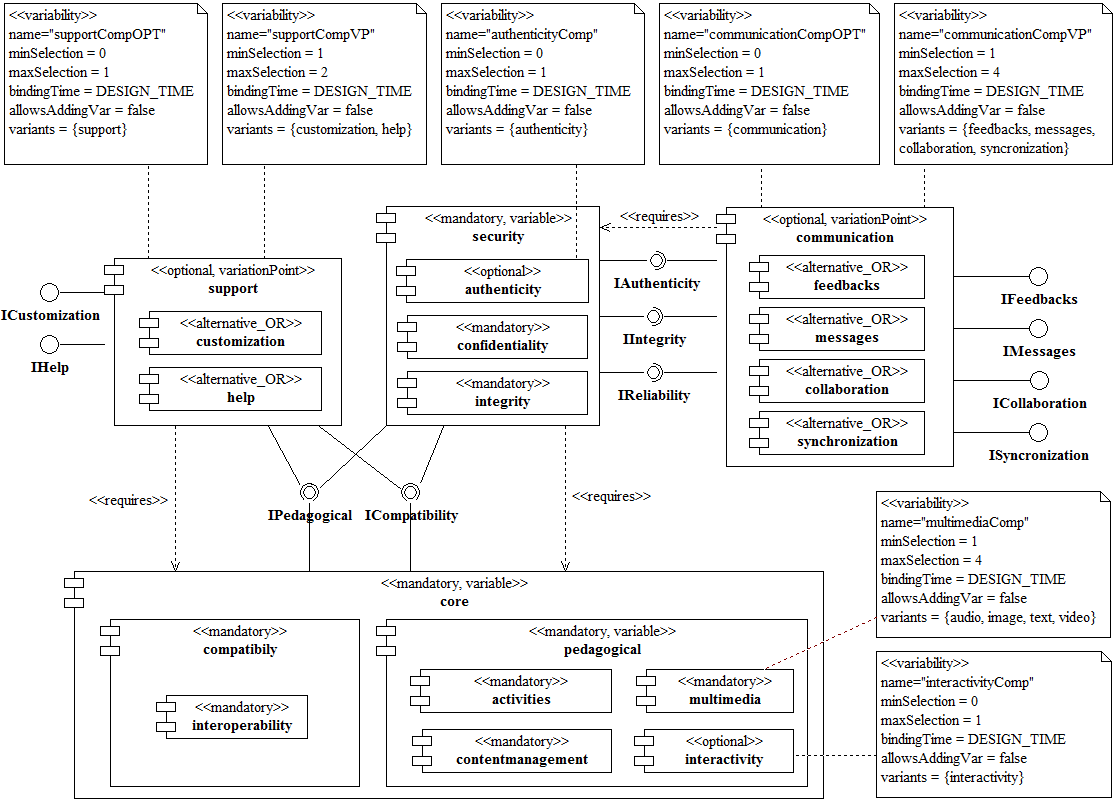
\includegraphics[scale=0.46]{figures/section3/MSPLDesign}
\caption{M-SPLearning SMarty-based Components Diagram.}
\label{figureMSPLDesign}
\end{figure}

%Por meio desse diagrama de componentes é possível visualizar todas as features concretas contempladas pela M-SPLearning. Os componentes resultantes foram rotuladas com os estereótipos característicos da abordagem SMarty. Esse diagrama permite a analise da quantidade de configurações possíveis aos aplicativos m-learning contemplados pela LPS.
Analyzing this component diagram it is possible to notice all concrete features covered by M-SPLearning. The resulting components are labeled with the characteristic stereotypes of SMarty approach. This diagram allows the analysis of the possible configurations for m-learning applications covered by the SPL.
%Por exemplo, o componente multimedia foi modelado como uma variabilidade (esteriótipo variability), ou seja, ele pode ser configurado para que uma LPS crie aplicações m-learning customizadas de acordo com suas configurações. Dessa forma, uma aplicação poderia ser configurada para possuir no mínimo um e no máximo quatro recursos multimédia (audio, image, text e video), conforme as notações "minSelection" e "maxSelection". Uma observação relevante é que qualquer componentes cujo filho foi modelado como uma variabilidade deve ser marcado como variável (esteriótipo variable).
For example, the \textit{multimedia} component was modeled with variability stereotype, ie it can be configured so that the SPL create specific m-learning applications according to your settings. Thus, a product can be configured to have among one and four \textit{multimedia} resources (audio, image, text and video), according to the notations ``minSelection" and ``maxSelection". Its important to highlight that any components formed for other components with variability should be tagged with the variable stereotype.

%Com ênfase no domínio explorado, os componentes pedagogical e communication se destacam, assim como seus requisitos. Nesse sentido, a maioria dos componentes pedagógicos são obrigatórios, com variabilidades possíveis em termos de interatividade e recursos multimídia (já explanada anteriormente). Por sua vez, os componentes agrupados em communication são alternativos, sendo que ao menos um deles deve agregar sua funcionalidade aos produtos gerados.
With emphasis on the explored domain, the \textit{pedagogical} and \textit{communication} components stand out, as well as your requirements. In this sense, most \textit{pedagogical} subcomponents are mandatories, with possible variabilities in terms of \textit{interactivity} and \textit{multimedia} features. In turn, the \textit{communication} subcomponents are alternatives, and at least one of them must provide its functionalities to the generated products.

%Também fica explícito o relacionamento de dependência entre os componentes modelados. Como definido anteriormente, o componente core unifica as features integralmente obrigatórias ao domínio m-learning, tornando-se necessário, direta ou indiretamente, aos componentes security, communication e support. A particularidade aqui fica por conta do componente communication, dependente do componente security, que por sua vez está relacionado com o componente core, fazendo com que o componente communication também tenha acesso a essa dependência. Isso garante a imposição arquitetônica de que todos os componentes parcialmente mandatórios ou opcionais dependam do componente core, que proverá as características fundamentais da M-SPLearning.
The dependency relationship between the modeled components also becomes explicit. As previously defined, the \textit{core} component unifies the mandatory features to m-learning domain, being necessary, directly or indirectly, to the \textit{security}, \textit{communication} and \textit{support} components. Particularly, the \textit{communication} component depends on the \textit{security} component, which in turn is related to the \textit{core} component. As a consequence, the \textit{communication} component also knows the \textit{core}.

%A partir do Projeto de Componentes aferidos pela LPS, torna-se possível a definição de um Plano de Produção que transforme as representações abstratas em produtos de software concretos, com suas respectivas variabilidades. A seção a seguir conclui a Análise de Domínio definida para a M-SPLearning.
Finally the Components Project, it is possible to define a Production Plan to transform the abstract representations in concrete software products, with their respective variabilities.

\subsubsection{Production Plan}

%O Plano de Produção prescreve como os produtos devem ser gerados a partir dos ativos centrais definidos para a LPS. Para isso, um diagrama de atividades usando a abordagem SMarty foi modelado, expondo as variabilidades possíveis durante o processo de criação de um produto (Figura \ref{figureMSPLProductionPlan}). Basicamente, este plano pode ser considerado um ativo central da M-SPLearning, assim como qualquer outro artefato que contribua para a criação sistemática de seus produtos. 
The Production Plan prescribes how the products should be generated from the core assets identified for the SPL. For this, an activity diagram using the SMarty approach was modeled, exposing the possible variabilities in the process of creating a product (Figure \ref{figureMSPLProductionPlan}). Basically, this plan can be considered a core asset of M-SPLearning, just like any other artifact that contributes to the systematic creation of their products.

\begin{figure}
\centering
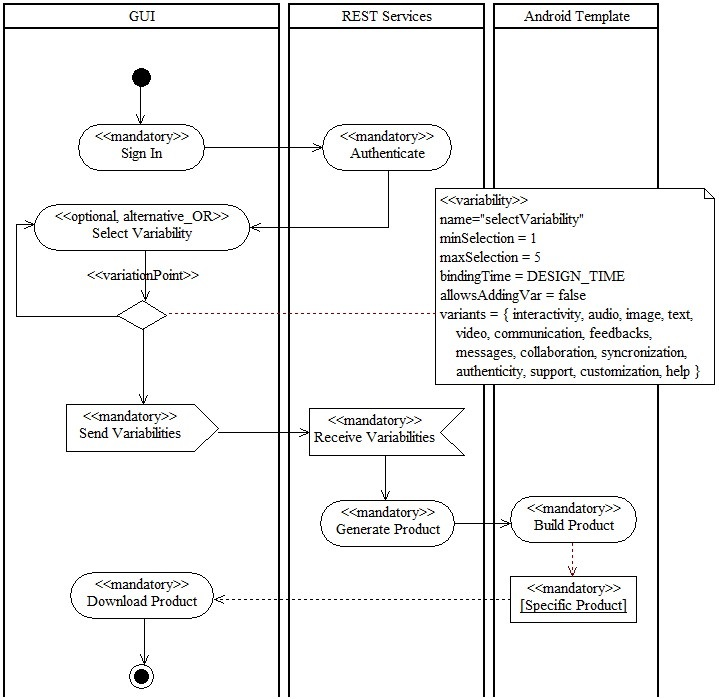
\includegraphics[scale=0.5]{figures/section3/MSPLProductionPlan}
\caption{M-SPLearning SMarty-based Production Plan.}
\label{figureMSPLProductionPlan}
\end{figure}

%O ponto de variação definido no plano de produção expõe todas as variabilidades elicitadas para a M-SPLearning. Desta forma, a customização dos produtos foi centralizada em um único ponto, agilizando o processo de configuração e geração dos aplicativos m-learning, provenientes da LPS proposta.
The variation point defined in the production plan exposes all variabilities elicited for M-SPLearning. Thus, the customization of the products was centralized at a single point, streamlining the configuration process and generation of m-learning applications by the SPL proposal.

%Cada raia do diagrama representa um módulo específico, sendo possível identificar algumas características arquiteturais da M-SPLearning. Uma das mais importantes neste sentido é a utilização do conceito de REpresentational State Tranfer (REST). Essa característica permite a criação e consumo de web services por meio do padrão Hypertext Transfer Protocol (HTTP), tornando viável a utilização de arquiteturas emergentes, como a Service-Oriented Architecture (SOA), também no contexto de aplicações móveis.
Each swimlane of the diagram represents a specific module, making it possible to identify some architectural characteristics of the M-SPLearning. One of the most important with this regard is the use of the REpresentational State Tranfer (REST) \cite{fielding00} architectural style. This concept allows the creation and consumption of web services using the Hypertext Transfer Protocol (HTTP), making possible the use of emerging software architectures such as Service-Oriented Architecture (SOA), also in the context of mobile applications.

%A seguir cada módulo representado no diagrama de atividades é sintetizado, considerando suas características técnicas e responsabilidades em termos práticos:
Next, each module represented in Figure \ref{figureMSPLProductionPlan} is synthesized considering its main characteristics in technical terms:

\begin{itemize}
    %Módulo que provê a interface gráfica dos usuários da LPS, ou seja, as representações visuais com as quais os usuários interagem para a geração dos produtos apoiados pela M-SPLearning. Neste módulo, é possível configurar as variabilidades e visualizar as similaridades, além de solicitar a geração de um produto personalizado. Este módulo foi implementado utilizando apenas tecnologias client-side, em especial HTML, JavaScript e CSS. A ideia foi demonstrar a interoperabilidade em uma arquitetura SOA, já que foram implementados todos os serviços usando REST, conforme o item a seguir.
	\item \textbf{\textit{Graphical User Interface (GUI):}} module responsible for providing the visual representations with which users interact to generate the products supported by M-SPLearning. In this module, the variabilities can be configured, allowing the generation of a customized product. This module was implemented using only client-side technologies, especially HTML, JavaScript and CSS. The idea was to demonstrate interoperability in a SOA architecture, since all services were implemented using REST.
	
	%Módulo desenvolvido a partir da abstração arquitetônica REST, que se caracteriza pelo uso de tecnologias e protocolos da web para a criação e entrega de serviços. Este estilo é totalmente aderente ao padrão arquitetural SOA e assegura a disponibilidade e consumo de web services de uma forma simples e eficiente. Este módulo corresponde à principal interface entre os produtos gerados pela M-SPLearning e suas features. Ele acessa um banco de dados remoto, onde todas as informações são armazenadas, incluindo as features (similaridades e variabilidades) especificadas via GUI. A centralização dos dados no módulo de serviços torna-o essencial para os outros (GUI e Android Template), uma vez que ambos consomem os web services disponibilizados por ele.
	\item \textbf{\textit{REST Services:}} module developed from the REST architectural abstraction, which is characterized by the use of technologies and protocols of the web for the creation and delivery of services. This style is fully adherent to the SOA architectural pattern and ensures the availability and consumption of web services in a simple and efficient way. This module is the main interface between the products generated by the M-SPLearning and its features. It accesses a remote database where all the information is stored, including features (similarities and variabilities) configured from the \textit{GUI}. The centralization of data in the \textit{REST Services} module is essential for other (\textit{GUI} and \textit{Android Template}), since both consume the web services provided by it.
	
	%Este módulo provê um template genérico para a customização dos produtos. Isso permite que um serviço, disponível no módulo REST Services, execute uma compilação personalizada de acordo com as variabilidades configurados no módulo GUI. O resultado é um Android Application Package (APK) com todas as features pré-configuradas, o que permite a instalação do produto customizado em qualquer dispositivo Android.
	\item \textbf{\textit{Android Template:}} module responsible for providing a generic template for the customization of products. This allows a service, available in \textit{REST Services} module, execute a custom build according to the variabilities configured in the \textit{GUI}. The result is an Android Application Package (APK) with all pre-configured features, allowing the installation of custom product on any Android device.
\end{itemize}

%Considerando a necessidade de construção de aplicações m-learning com maior qualidade e reúso, os esforços para o desenvolvimento de LPS que lidam com aspectos SOA ganharam especial importância no contexto móvel. A adoção de uma abordagem SOA torna-se cada vez mais relevante, principalmente porque torna mais fácil e flexível a construção de suas aplicações, promovendo interoperabilidade e reutilização, o que corrobora com as definições arquiteturais propostas no plano de produção.
Considering the need of building m-learning applications with higher quality and reuse, efforts for the development of SPL dealing with SOA aspects gained special importance in the mobile context \cite{marinho10, nascimento11}. The adoption of an SOA approach becomes increasingly important, especially because it makes easy and flexible to build their applications, promoting interoperability and reuse, which agrees with the architectural definitions proposed in the production plan.

%A M-SPLearning foi elaborada a partir de um processo baseado em práticas e conceitos relevantes no âmbito da Engenharia de Software. Com isso, a M-SPLearning utilizou um processo sequencial para sua definição, abordando as dificuldades da análise de elementos do domínio e as definições arquiteturais necessárias para sua implementação proativa. A próxima seção trata da atividade primária subsequente, a Engenharia de Aplicação.
M-SPLearning was elaborated from a process based on relevant practices and concepts in software engineering. Thus, M-SPLearning has used an incremental process for its definition, addressing the difficulties of domain analysis and the necessary architectural definitions for a proactive implementation. The next section deals with the subsequent SPL activity, the AE.

\subsection{Application Engineering}\label{section32}

%Esta atividade depende essencialmente dos artefatos de saída da Engenharia de Domínio, que agora atuam como artefatos de entrada. A partir dos ativos gerados, um conjunto específico de features foi selecionado para a implementação da M-SPLearning. Essa redução de escopo foi definida com o objetivo de viabilizar a avaliação experimental da M-SPLearning. Dessa forma, com um número reduzido de features, foi possível implementar e avaliar a LPS em um prazo aceitável.
This activity depends on the output artifacts of DE, which now act as input devices. Using these artifacts, a specific set of features was selected for the implementation of M-SPLearning. This reduction in scope was defined in order to enable the experimental evaluation of the M-SPLearning. Thus, with a limited number of features, it was possible to implement the SPL in 188 hours, enabling even their experimental evaluation.

%No contexto deste trabalho, as features relacionadas às atividades pedagógicas e de segurança foram priorizadas e implementadas. O motivo dessa escolha é que as features em questão representam os requisitos funcionais mínimos de uma aplicação m-learning, são eles: (i) Pedagogical: inclui a realização de atividades educacionais através do gerenciamento de conteúdos interativos e recursos multimédia; (ii) Security: agrega em termos de confidencialidade e integridade dos dados, além da possibilidade de autenticação dos usuários; e (iii) Communication: incluiu apenas a feature relacionada à sincronização de dados.
In the context of this work, the features related to teaching and security activities were prioritized and implemented. The reason for this choice is that such features are the minimum functional requirements of a m-learning application: (i) \textit{Pedagogical}: includes conducting educational activities through the management of interactive and multimedia content; (ii) \textit{Security}: provides confidentiality and integrity of data, added by the ability to authenticate users; and (iii) \textit{Communication}: includes the feature related to data synchronization.

%Tecnicamente, a M-SPLearning apresenta a visão lógica de uma LPS definida para configuração e geração de aplicações m-learning na plataforma Android. Sua implementação foi feita predominantemente em Java e seu código fonte pode ser consultado a partir do repositório open source GitHub.
In technical terms,  M-SPLearning presents the logical view of an SPL defined for configuration and generation of m-learning applications on the Android platform. Its implementation was made predominantly in Java and its source code is available\footnote{http://github.com/falvojr/msplearning} on GitHub open source repository.

%Por definição, a Engenharia de Aplicação instancia os ativos centrais de uma LPS para geração de produtos específicos. Para isso, o plano de produção, até então abstrato, foi utilizado para a construção de seus respectivos módulos concretos. No contexto desta atividade, o módulo GUI foi inevitavelmente o mais explorado, porque todos os produtos são gerados através dele.
By definition, the AE instantiates the core assets of SPL to generate specific products. For this, the production plan was used to build the respective concrete modules. In the context of this activity, the \textit{GUI} module is inevitably the most exploited, because all products are generated therethrough.

%A primeira interação entre usuário e a M-SPLearning ocorre em uma página inicial web. Nela, os usuários podem registrar-se e, posteriormente, autenticar-se na aplicação. Essa interface visual também introduz o domínio e os principais objetivos da M-SPLearning, contextualizando seus usuários. Outro aspecto relevante foi a construção de suas páginas web completamente baseadas no conceito de layouts responsivos, o que, dentre outras tendências, tornou a representação visual da LPS ainda mais dinâmica e flexível. A Figura \ref{figureMSPLWebLogin} expõe tais características.
The first interaction between the user and M-SPLearning occurs in a web home page. Therein, users can sign up and then log into the application. This interface also introduces the domain and the main objectives of M-SPLearning. Another important aspect refers the construction of the web pages completely based on the concept of responsive layouts, which makes the visual representation of SPL even more dynamic and flexible. 

%Figure \ref{figureMSPLWebLogin} presents such characteristics.
%
%\begin{figure}
%\centering
%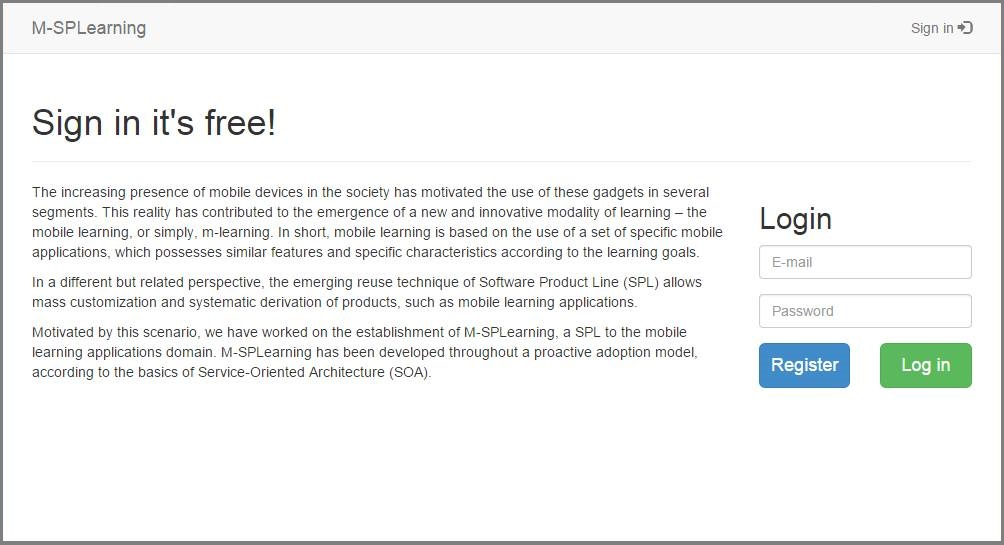
\includegraphics[scale=0.4]{figures/section3/MSPLWebLogin}
%\caption{M-SPLearning GUI Login.}
%\label{figureMSPLWebLogin}
%\end{figure}

%Com um usuário devidamente autenticado, a interface resultante é a caracterização mais evidente da M-SPLearning, já que possibilita o gerenciamento visual das variabilidades disponibilizadas pela LPS. Neste ponto, o usuário, por exemplo um professor, simplesmente realiza alguns cliques para geração de um produto específico, criando, assim, um APK com uma aplicação m-learning instalável em qualquer dispositivo Android.
With an authenticated user, the resulting interface is the most evident characterization of M-SPLearning, as it enables the visual management of variabilities provided by SPL. At this point, the user, for example a teacher, simply performs a few clicks to generate a specific product, which creates an APK that encapsulates a custom m-learning application for any Android device. The page for performing this procedure is illustrated in Figure \ref{figureMSPLWebGeneration}, which also shows the visual interface for managing the products generated by M-SPLearning. Furthermore, it is important to note that the variabilities related to features prioritized during this implementation can be configured in the products generation.

%A página para a realização desse procedimento é ilustrado pela Figura 1, que também apresenta a interface visual para o gerenciamento dos produtos gerados através da M-SPLearning. Além disso, é importante observar que as variabilidades relacionadas às features priorizadas durante essa implementação podem ser configuradas na geração dos produtos.

\begin{figure}[!ht]
\centering
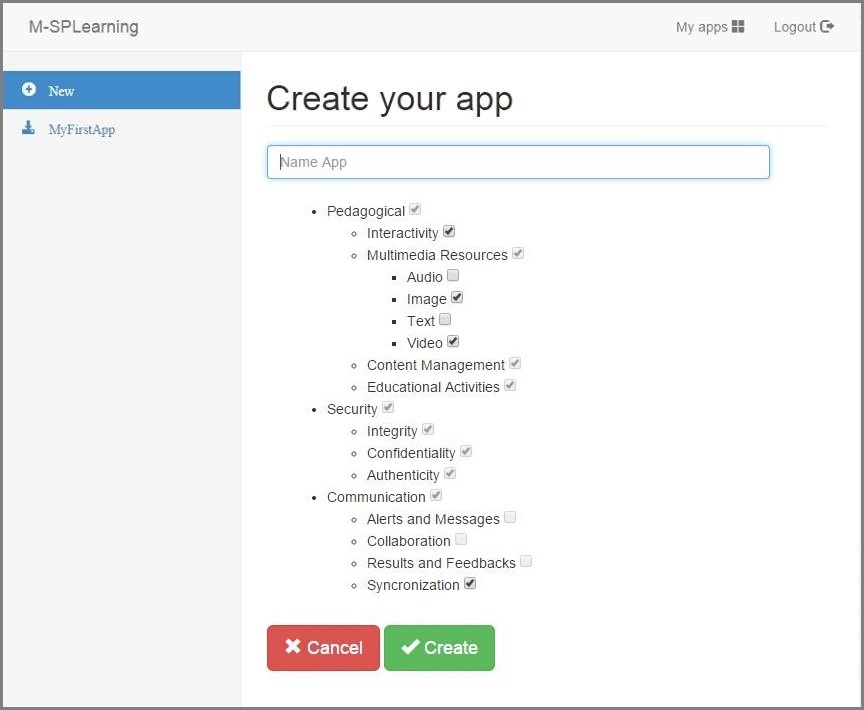
\includegraphics[scale=0.45]{figures/section3/MSPLWebGeneration}
\caption{M-SPLearning GUI Product Generation.}
\label{figureMSPLWebGeneration}
\end{figure}

%Ao solicitar a geração de um APK, os módulos REST Service e Android Template são acionados simultaneamente. Essa integração resulta na criação de um produto aderente às variabilidades selecionadas pelo usuário. A partir deste momento a aplicação m-learning gerada pode ser instalada no dispositivo móvel de qualquer professor ou aluno, que deve se registrar na aplicação móvel, caso a feature Authentication tenha sido selecionada durante a criação do APK.
When request the generation of a APK the \textit{REST Services} and \textit{Android Template} modules are triggered simultaneously. This integration results in the creation of a adherent product to user selected variabilities. Thus, the m-learning application generated can be installed on the Android device of any teacher or student, who must register with the mobile application if the feature \textit{Authentication} has been selected when creating the APK.

%A Figura 1 mostra dois produtos gerados com as variabilidades Authenticity e Interactivity configuradas de formas diferentes, nas quais: (a) o produto foi configurado apenas com a feature Authenticity; e (b) o produto foi gerado com ambas as variabilidades, o que explica o formulário de autenticação com a possibilidade de interação com algumas redes sociais.
Figure \ref{figureMSPLLogin} illustrates two products generated with \textit{Authenticity} and \textit{Interactivity} variabilities configured in different ways: (a) the product was configured with only the Authenticity feature; and (b) the product was generated with both variabilities, which explains the authentication form with the possibility of interaction with some social networking.

\begin{figure}[!ht]
\centering
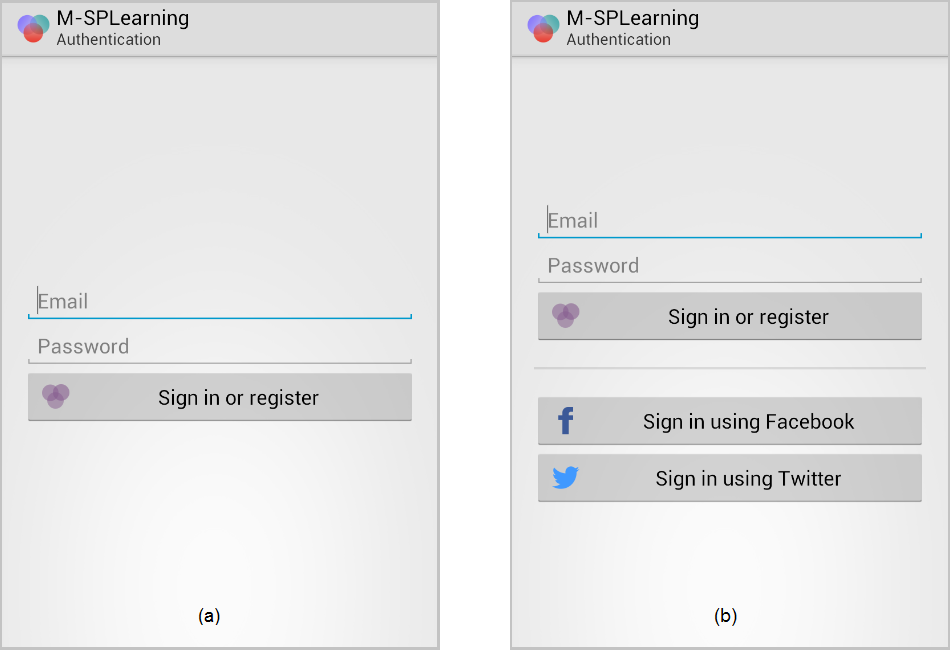
\includegraphics[scale=0.35]{figures/section3/MSPLLogin}
\caption{M-SPLearning Product Login -- Configurations of the features:\newline(a) \textit{Authenticity}; and (b) \textit{Authenticity} and \textit{Interactivity}.}
\label{figureMSPLLogin}
\end{figure}

%Observando a Figura 1 nota-se que o botão comum aos produtos também prevê a possibilidade de registro de um novo usuário. Para isso, o usuário deve apenas preencher seu e-mail e senha nos campos disponíveis para que a aplicação m-learning verifique a existência de seu usuário. Em caso negativo, o formulário de cadastro é exibido já com as informações digitadas preenchidas (Figura 2).
According to Figure \ref{figureMSPLLogin}, the common button to products also provides the possibility of registering a new user. To do this, one should fill his/her email and password in the fields available for the application to verify if the user exists (Figure \ref{figureMSPLRegister} (a)). If not, the registration form is displayed with the information previously typed (Figure \ref{figureMSPLRegister} (b)).

\begin{figure}[!ht]
\centering
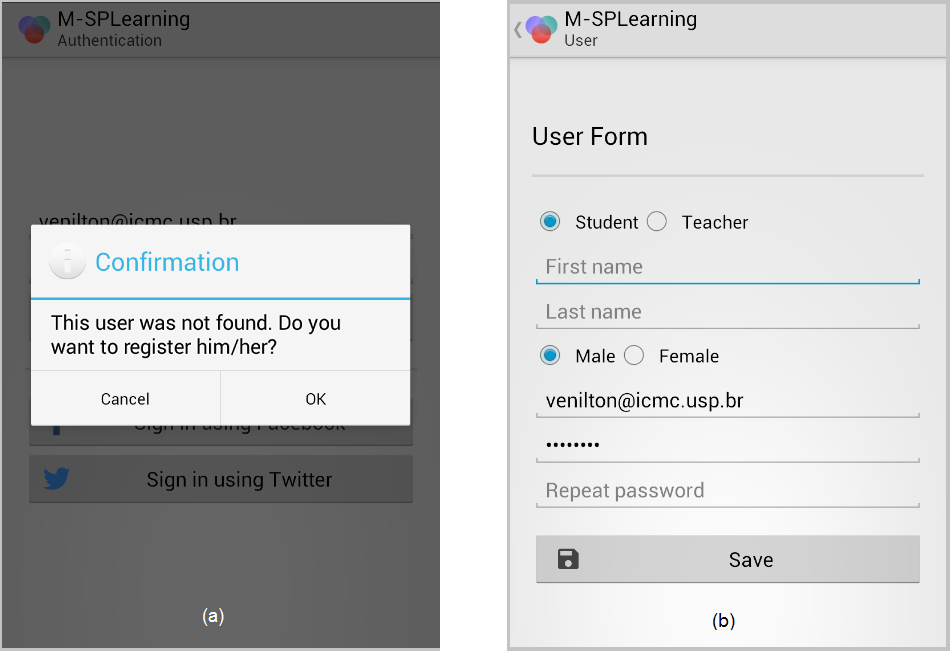
\includegraphics[scale=0.35]{figures/section3/MSPLRegister}
\caption{M-SPLearning Product Registration -- Steps for user registration:\newline(a) Confirmation message; and (b) Registration Form.}
\label{figureMSPLRegister}
\vspace{0.65cm}
\end{figure}

%O formulário de cadastro de usuário permite a seleção do tipo de acesso: professor ou aluno. Por motivos de segurança, todos os usuários registrados devem ser aprovados pelo usuário que gerou o APK. Para isso, no momento de criação da aplicação o usuário é associado a mesma com perfil administrativo. Esse aspecto deixa evidente a feature "Content Management", uma vez que cada perfil de usuário prevê acessos específicos e bem definidos. A Figura 1 ilustra um cenário possível, em que: (a) apresenta a visão de um professor; e (b) apresenta a visão de um aluno, com o adendo de que neste exemplo nenhum conteúdo educacional foi incluído, tendo em vista que o acesso a esta funcionalidade está desabilitado.
The user registration form allows the selection of the type of access: teacher or student. For security reasons, all registered users must be approved by the user who generated the APK. For this, at the time of creation of the APK the user is associated with administrative profile. This aspect makes clear the feature \textit{Content Management}, since each user profile provides specific and well-defined accesses. Figure \ref{figureMSPLDashboardApp} illustrates a possible scenario presenting: (a) the teacher's views; and (b) the student's view, but with no content, since the access to this feature is disabled.

\begin{figure}[!ht]
\centering
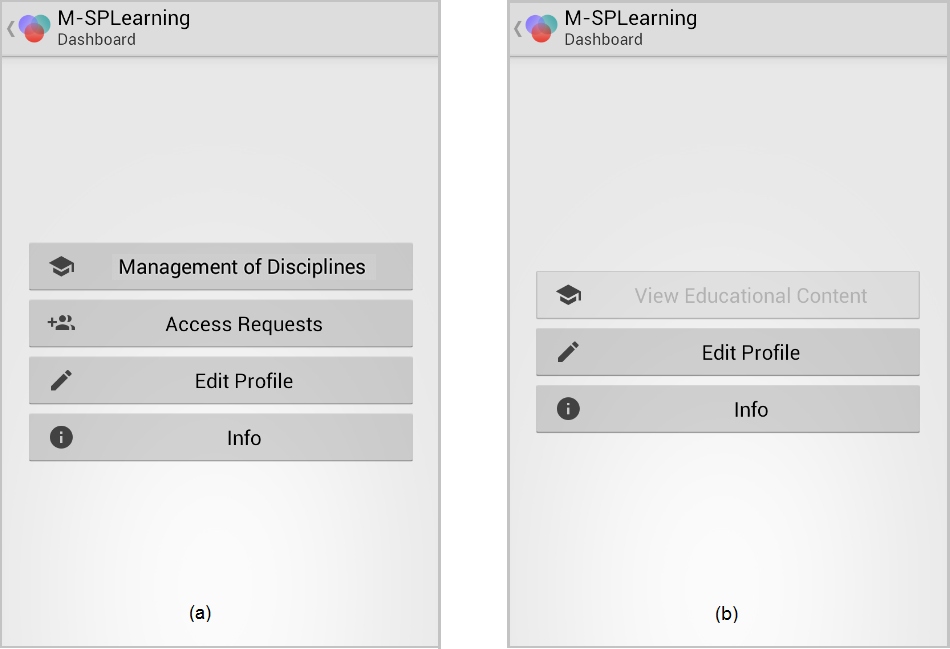
\includegraphics[scale=0.35]{figures/section3/MSPLDashboardApp}
\caption{M-SPLearning Product Dashboard -- Access Profiles:\newline(a) Teacher; and (b) Student.}
\label{figureMSPLDashboardApp}
\end{figure}

%Com um usuário devidamente autenticado e com suas respectivas funcionalidades fornecidas, a aplicação m-learning está pronta para armazenamento e compartilhamento do seu principal ativo, os conteúdos educacionais. Neste sentido, o professor pode cadastrar suas disciplinas, lições e finalmente o conteúdo de cada uma delas. Essas funcionalidades representam um contexto de uso das features Educational Activities e Multimedia Resources, também representadas pela Figura 1.
With user properly authenticated, the m-learning application is ready for storage and sharing of its main asset, the educational content. In this sense, the teacher can register his/her courses, lessons and finally the content of each lesson. These functionalities are an usage sample of the \textit{Educational Activities} and \textit{Multimedia Resources}, as shown in Figure \ref{figureMSPLEducationalContent}.

\begin{figure}[!ht]
\centering
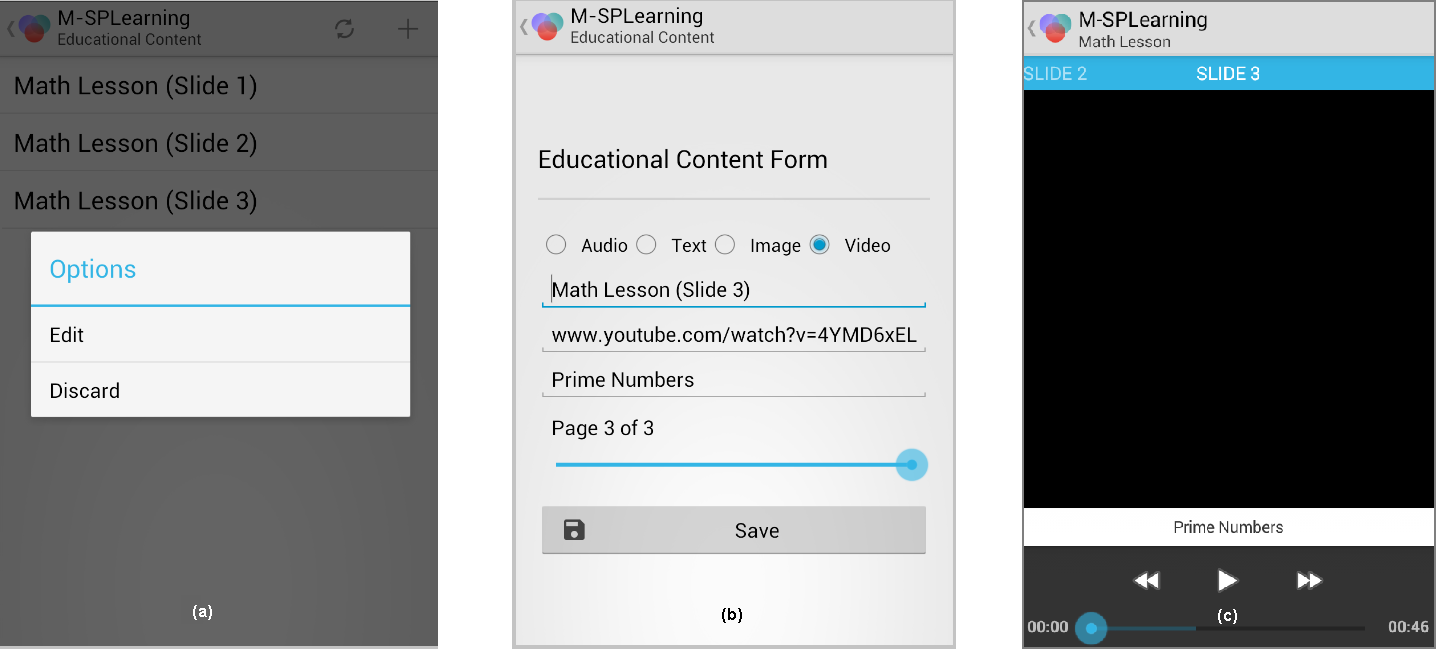
\includegraphics[scale=0.35]{figures/section3/MSPLEducationalContent}
\caption{M-SPLearning Product Educational Content Management:\newline(a) Listing of educational content and context menu; (b) Editing form; and (c) Displaying video content.}
\label{figureMSPLEducationalContent}
\end{figure}

%De acordo com as features disponibilizadas pela M-SPLearning, nota-se a possibilidade de inclusão de conteúdos educacionais dos seguintes tipos: áudio, texto, imagem e vídeo. No exemplo apresentado, a opção de vídeo está selecionada, o que provê ao professor a inclusão de uma URL para a disponibilização do vídeo desejado aos alunos que compartilham essa aplicação.
According to the features provided by M-SPLearning, it is possible to include content of the following types: audio, text, image and video. %In the example shown, the video is selected, providing to the teacher the inclusion of an URL to the availability of the desired video students to share this application.
%Assim, os alunos visualizam os conteúdos educacionais incluídos pelos professores cadastrados na aplicação, obtendo assim acesso centralizado a sua gama de conteúdos educacionais. A Figura 1 ilustra, na perspectiva de aluno, um exemplo de conteúdo educacional do tipo vídeo.
The Figure \ref{figureMSPLEducationalContent} (c) illustrates an example of a video feature in the student perspective.

%É importante observar que foi possível incluir os requisitos previamente definidos para a construção de uma LPS. A concepção da M-SPLearning envolveu desde a análise e projeto até a implementação funcional da proposta desta pesquisa. A avaliação formal da M-SPLearning, junto de sua abordagem e principais resultados, são descritos na Seção \ref{section4}.
It is important to note that it was possible to include the requirements previously set for the construction of an SPL. The design of the M-SPLearning involved from analysis and design to functional implementation. A formal evaluation of the M-SPLearning, along with this approach and main results is described in Section \ref{section4}.

\section{M-SPLearning Experimental Evaluation}\label{section4}

This section presents the experimental evaluation of M-SPLearning with respect to time-to-market and quality improvement. M-SPlearning was compared with software singular development methodology. The guidelines proposed by Jedlitschka et al. \cite{jedlitschka07} were followed to report controlled experiments.

\subsection{Motivation}\label{sub:motivation}


The choice in the adoption of new technologies or approaches used in development process depends on which aspects of quality and benefits are desired. Despite the fact of many approaches have been established in the literature, there are many issues to be solved about them to conduct a suitable adoption in both industry and academic environments. Experimental evaluations may bring the light in the identification of evidences from quality aspects and benefits in these approaches, supporting the choice of them. In some cases, the collected evidence may still supports the correction of problems identified during the experimental evaluations, allowing the improvement of the proposals.

Therefore, to collect initial evidence in two crucial development perspectives, time-to-market and quality in terms of number of faults, the experimental evaluation of the M-SPlearning is presented.

\subsubsection{Research Objectives}\label{sub:object}

The goal of the experiment was to \textbf{compare} the singular software development methodology (SSD) and the software product line (SPL) methodology, \textbf{for the purpose of} identifying the most efficient, \textbf{with respect to} the time spent for creating software products (time) and the number of faults of the created software products, \textbf{in the context of} practitioners from industry.


\subsection{Experimental Design}\label{sub:design}

This section provides the experimental design and procedures for supporting future replications.

\subsubsection{Goals}

Based on the research objective two research questions (R.Q.) were stated:

\textbf{R.Q.1} Which methodology is more efficient with respect to time-to-market, SSD or SPL?

\textbf{R.Q.2} Which methodology showed more quality in terms of the number of faults in the created software product, SSD or SPL?

\subsubsection{Hypotheses}

Two sets of hypotheses were defined to be tested, each of them related with its respective research questions (R.Q.1 and R.Q.2):

\textbf{R.Q.1 hypotheses:} time-to-market

	\begin{itemize}
	
	\item \textbf{Null Hypothesis ($H_{0}$)}: there is no significant difference of time-to-market between SSD and SPL.
	
	$H_{0}$ : $\mu$(\textit{t(SSD)}) =  $\mu$(\textit{t(SPL)});
	
	\item \textbf{Alternative Hypothesis ($H_{1}$)}: SSD has less time-to-market than SPL.
	
	$H_{1}$ : $\mu$(\textit{t(SSD)}) $<$ $\mu$(\textit{t(SPL)});
		
	
	\item \textbf{Alternative Hypothesis ($H_{2}$)}: SSD has more time-to-market than SPL.
	
	$H_{2}$ :  $\mu$(\textit{t(SSD)}) $>$ $\mu$(\textit{t(SPL)}).		
	
	\end{itemize}	

\textbf{R.Q.2 hypotheses:}
quality in terms of the number of faults
	\begin{itemize}
	
	\item \textbf{Null Hypothesis ($H_{0}$)}: there is no significant difference between SSD and SPL with regard to quality in terms of number of faults in the software products created.
	
	$H_{0}$ : $\mu$(\textit{d(SSD)}) =  $\mu$(\textit{d(SPL)});
	
	\item \textbf{Alternative Hypothesis ($H_{1}$)}: SSD has greater number of faults than SPL.
	
	$H_{1}$ : $\mu$(\textit{d(SSD)}) $>$ $\mu$(\textit{d(SPL)});
		
	\item \textbf{Alternative Hypothesis ($H_{2}$)}: SSD has minor number of faults than SPL.
	
	$H_{2}$ :  $\mu$(\textit{d(SSD)}) $<$ $\mu$(\textit{d(SPL)}).		
	
	\end{itemize}

\subsubsection{Variables}

Dependent variables are the mean of time ($t$) and faults ($f$), defined as follows:

\small

\begin{equation}\label{eq:1}
\mu{(t)}=(\Sigma xi)/n, i = 1..n
\end{equation}
\begin{equation}\label{eq:2}
\mu{(f)}=(\Sigma yi)/n, i = 1..n
\end{equation}
\normalsize 
where:
\begin{itemize}
\item \textit{t} is the time of implementation (minutes);
\item \textit{f} is the number of faults;
\item \textit{xi} is the time of implementation of participant i;
\item \textit{yi} is the number of faults detected in the implementation of participant i; and
\item \textit{n} is the total of participants in the experiment.
\end{itemize}
\normalsize

Independent variables are the development methodology, which is a factor with two treatments (SSD and SPL), and the software product configuration for mobile learning platform, which is a factor with two treatments: product 1 (P1) and product 2 (P2). Table \ref{tab:variables} presents the description of dependent and independent variables.

%\begin{landscape}

\begin{table}[h]
\caption{\label{tab:variables}Dependent and Independent Variables Description.}
\centering
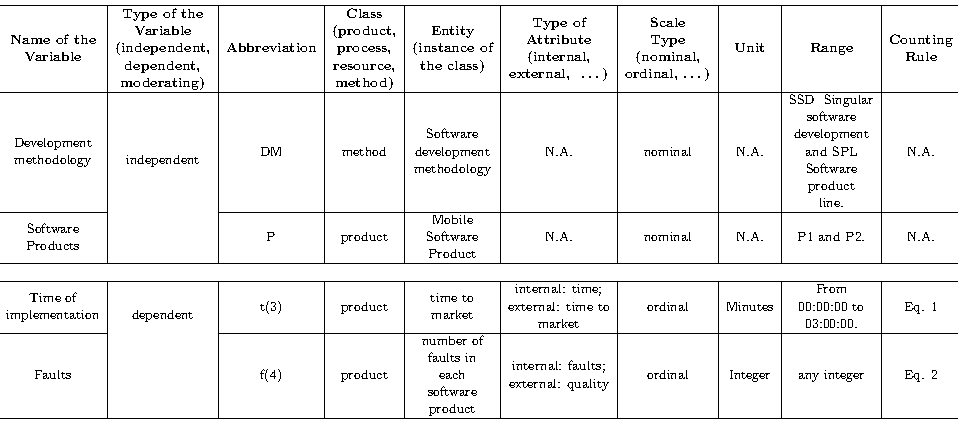
\includegraphics[scale=0.85]{figures/section4/tab_n.pdf}



%\resizebox{1.2\textwidth}{!}{
%\small
%\begin{tabular}{cccccccccc}
%\multicolumn{1}{l}{}                                                                         & \multicolumn{1}{l}{}                                                                                                                      & \multicolumn{1}{l}{}                                 & \multicolumn{1}{l}{}                                                                                                        & \multicolumn{1}{l}{}                                                                                           & \multicolumn{1}{l}{}                                                                                                        & \multicolumn{1}{l}{}                                                                                            & \multicolumn{1}{l}{}                                                                & \multicolumn{1}{l}{}                                                                                                                             & \multicolumn{1}{l}{}                                              \\ \hline
%\multicolumn{1}{c|}{\textbf{\begin{tabular}[c]{@{}c@{}}Name of the\\ Variable\end{tabular}}} & \multicolumn{1}{c|}{\textbf{\begin{tabular}[c]{@{}c@{}}Type of the\\ Variable\\ (independent, \\ dependent, \\ moderating)\end{tabular}}} & \multicolumn{1}{c|}{\textbf{Abbreviation}}           & \multicolumn{1}{c|}{\textbf{\begin{tabular}[c]{@{}c@{}}Class\\ (product, \\ process, \\ resource, \\ method)\end{tabular}}} & \multicolumn{1}{c|}{\textbf{\begin{tabular}[c]{@{}c@{}}Entity\\ (instance of \\ the class)\end{tabular}}}      & \multicolumn{1}{c|}{\textbf{\begin{tabular}[c]{@{}c@{}}Type of \\ Attribute \\ (internal, \\ external, \ \ldots)\end{tabular}}} & \multicolumn{1}{c|}{\textbf{\begin{tabular}[c]{@{}c@{}}Scale\\  Type \\ (nominal, \\ ordinal,\ \ldots)\end{tabular}}} & \multicolumn{1}{c|}{\textbf{Unit}}                                                  & \multicolumn{1}{c|}{\textbf{Range}}                                                                                                              & \textbf{\begin{tabular}[c]{@{}c@{}}Counting \\ Rule\end{tabular}} \\ \hline
%\multicolumn{1}{c|}{\begin{tabular}[c]{@{}c@{}}Development\\ methodology\end{tabular}}       & \multicolumn{1}{c|}{\multirow{2}{*}{independent}}                                                                                         & \multicolumn{1}{c|}{DM}                              & \multicolumn{1}{c|}{method}                                                                                                 & \multicolumn{1}{c|}{\begin{tabular}[c]{@{}c@{}}Software\\ development \\ methodology\end{tabular}}             & \multicolumn{1}{c|}{N.A.}                                                                                                   & \multicolumn{1}{c|}{nominal}                                                                                    & \multicolumn{1}{c|}{N.A.}                                                           & \multicolumn{1}{c|}{\begin{tabular}[c]{@{}c@{}}SSD – Singular \\ software \\ development \\ and SPL \\ Software \\ product\\  line.\end{tabular}} & N.A.                                                              \\ \cline{1-1} \cline{3-10} 
%\multicolumn{1}{c|}{\begin{tabular}[c]{@{}c@{}}Software\\ Products\end{tabular}}             & \multicolumn{1}{c|}{}                                                                                                                     & \multicolumn{1}{c|}{P}                               & \multicolumn{1}{c|}{product}                                                                                                & \multicolumn{1}{c|}{\begin{tabular}[c]{@{}c@{}}Mobile\\ Software \\ Product\end{tabular}}                      & \multicolumn{1}{c|}{N.A.}                                                                                                   & \multicolumn{1}{c|}{nominal}                                                                                    & \multicolumn{1}{c|}{N.A.}                                                           & \multicolumn{1}{c|}{P1 and P2.}                                                                                                                  & N.A.                                                              \\ \hline
%\multicolumn{10}{c}{}                                                                                                                                                                                                                                                                                                                                                                                                                                                                                                                                                                                                                                                                                                                                                                                                                                                                                                                                                                                                                                                                                       \\ \hline
%\multicolumn{1}{c|}{\begin{tabular}[c]{@{}c@{}}Time of \\ implementation\end{tabular}}       & \multicolumn{1}{c|}{\multirow{2}{*}{dependent}}                                                                                           & \multicolumn{1}{c|}{\begin{equation}t\end{equation}} & \multicolumn{1}{c|}{product}                                                                                                & \multicolumn{1}{c|}{\begin{tabular}[c]{@{}c@{}}time to\\ market\end{tabular}}                                  & \multicolumn{1}{c|}{\begin{tabular}[c]{@{}c@{}}internal: time;\\  external: time to \\ market\end{tabular}}                 & \multicolumn{1}{c|}{ordinal}                                                                                    & \multicolumn{1}{c|}{Minutes} & \multicolumn{1}{c|}{\begin{tabular}[c]{@{}c@{}}From \\ 00:00:00 to \\03:00:00.\end{tabular}}                                                                                                                   & \begin{tabular}[c]{@{}c@{}}Eq. 1\end{tabular}           \\ \cline{1-1} \cline{3-10} 
%\multicolumn{1}{c|}{Faults}                                                                  & \multicolumn{1}{c|}{}                                                                                                                     & \multicolumn{1}{c|}{\begin{equation}f\end{equation}} & \multicolumn{1}{c|}{product}                                                                                                & \multicolumn{1}{c|}{\begin{tabular}[c]{@{}c@{}}number of\\ faults in\\ each\\ software\\ product\end{tabular}} & \multicolumn{1}{c|}{\begin{tabular}[c]{@{}c@{}}internal: faults;\\ external: quality\end{tabular}}                          & \multicolumn{1}{c|}{ordinal}                                                                                    & \multicolumn{1}{c|}{Integer} & \multicolumn{1}{c|}{any integer}                                                                                                                 & \begin{tabular}[c]{@{}c@{}}Eq. 2\end{tabular}           \\ \hline
%
%\end{tabular}
%}
\end{table}
%\end{landscape}

Time-to-market is the average time spent for the implementation of a software product with a specific group of variabilities of M-SPLearning. With regard to the number of faults, the implemented products were tested using the concept of test cases \cite{craig02}. Thus, it was possible to quantify the mean of defects of products. Such metrics are relevant because they are directly related to time-to-market and quality of the m-learning applications.

\subsubsection{Participants}

In our study, the participants were employee volunteers from a Brazilian software development industry. All of them had, at least, one year of experience, with development background in Java, Microsoft .NET and/or PHP.

The reduced number of practitioners led us to apply a non-random selection. The random capacity was applied at the assignment of the development methodology and the software product to each participant. 

Block classification was defined by the two factors with two treatments, which were interspersed in four set of documents. Thus, the population was divided into four blocks by means of a draw. The balancing was applied in the tasks, that were assigned in equal numbers to a similar number of participants.

Participants were randomly separated into the following groups:

\begin{itemize}
\item \textbf{First Group:} focused in SSD with P1, them in SPL with P2;

\item \textbf{Second Group:} focused in SPL with P1, and in SSD with P2;

\item \textbf{Third Group:} focused in SSD with P2, and with SPL with P1; and

\item \textbf{Fourth Group:} focused in SPL with the P2, and with SSD with P1;
\end{itemize}

\subsubsection{Objects}

Among a total of 30 features and diferent configurations, two educational software products configurations for mobile learning platform (Android) were taken into consideration to apply the SSD and SPL methodologies which are: one for image (P1) and another for video resource (P2).

\subsubsection{Instrumentation}

The experiment was supported by a set of instruments: (i) similar desktop computers with all necessary tools (Eclipse IDE and plugins); (ii) the consent term to the experimental study; (iii) a characterization questionnaire; (iv) use case, component and sequence UML diagrams; (v) interface messages; (vi) database model; (vii) one project base; (viii) composed of the similarities of the products; (ix) the experimental forms for SSD and SPL, randomly distributed and feedback questionnaire.

\subsubsection{Data Collection and Analysis Procedures}

The main assessment tools were the products developed based in two software specifications (P1 and P2) for mobile learning platform (Android).

Based on the catalog of requirements (Section \ref{section2}), the M-SPLearning was designed with a total of 30 features from m-learning applications having 16 mandatory features and 14 optional features. A specific niche of features was used for our experimental evaluation, where the variabilities related to multimedia resources let one to create up to 15 different products (as represented by Figure \ref{figureMSPLFeatureModel}). Two specifics products (P1 and P2) were specified and implemented using both SSD and SPL methodologies. Figure \ref{fig:prod} represents the nuances between products generated for the video feature.


\begin{figure*}[t]
\centering
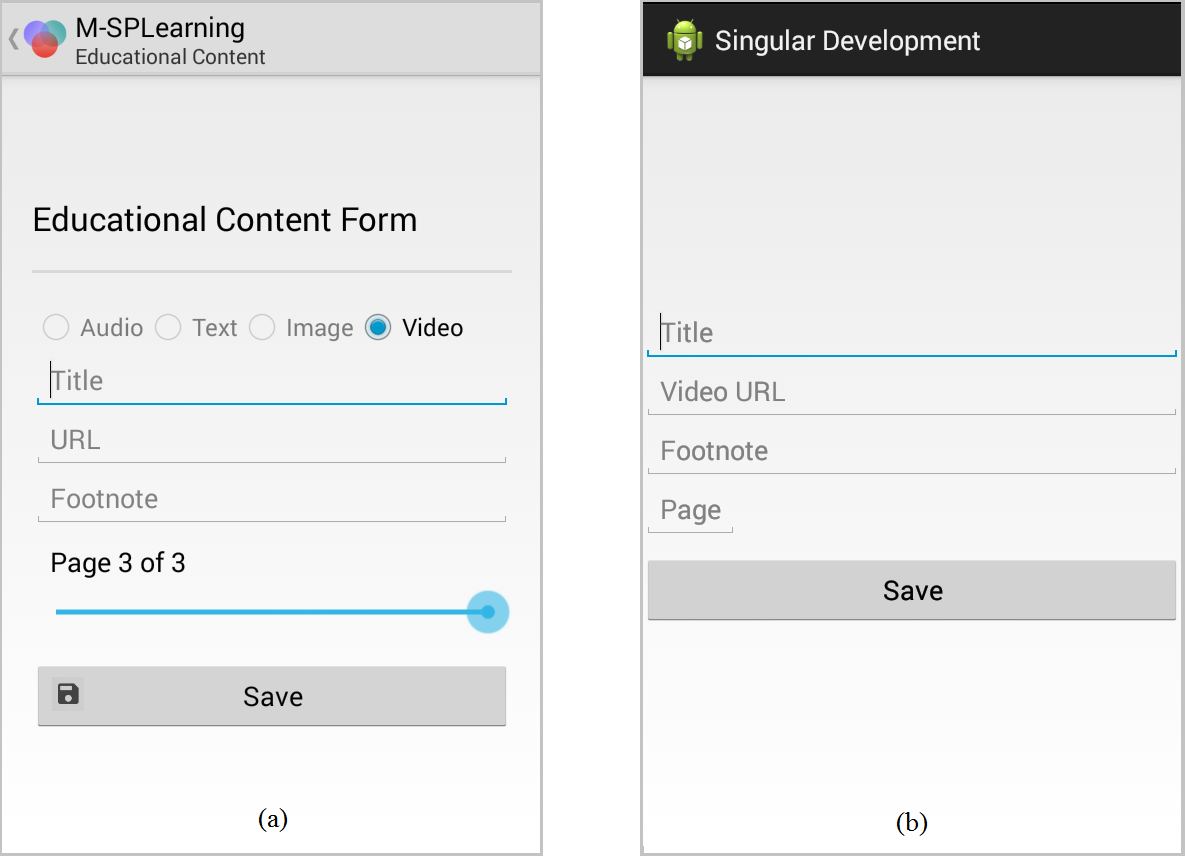
\includegraphics[scale=0.275]{figures/section4/prod.png}
\centering
\caption{Two Video Products (P1) Developed in the Experimental Execution with a) SPL and b) SDD.}
\label{fig:prod}
\end{figure*}


To collect the data for the analysis of time-to-market, the initial and final time of implementation process for P1 and P2, was registered individually in the experimental form to be calculated in Equation \ref{eq:1}. On the other hand, for the analysis of quality, each of 15 finished developed products were tested and the number of faults was collect to compare the use of SPL and SDD methodologies by means of the Equation \ref{eq:2}.

\subsubsection{Validity Evaluation}

A pilot project was conducted with two pratictioners from industry, evaluating the study instrumentation and allowing to estimate the duration of the training and execution sessions. The pilot results and its participants were not used in the final execution and data analysis of the experiment.

\subsection{Execution}\label{sub:execution}

This section presents how the experimental plan (design) was enacted.

\subsubsection{Sample}

The sample was composed of a total of 21 pratictioners who participated in the training session. However, 18 participants contributed in the experimental execution, due the unavailability of 3 volunteers in the execution day.

\subsubsection{Preparation}

The participants were trained with regard to essential concepts of Android development for SSD and SPL with the Eclipse IDE. The training lasted three days. The knowledge of the participants was evaluated with essays in the end of each training session. In the fourth day, the experiment was performed.

\subsubsection{Data Collection Performed}

The procedures adopted for data collection were:

\begin{enumerate}

\item the participants present in three trainning sessions, one per day, lasting 4 hours, in industrial environment;

\item the participants were divided in four groups by means of a draw;
\item the experimenter gave the participant a set of documents: the UML diagram models, dataset model, interface message specification for each product, such as the material used in training session. Each one was allocated in a desktop computer, with all requirements to develop the software product. Besides, each participant received an experimental form where they registered the spending time to development process to be analysed.
\item the participant reads each given document;
\item the experimenter explains the given documents;
\item the participant reads and clarifies possible doubts about the products specifications; and
\item finally, each participant received and used two randomly drawn methodologies to development a requested m-learning product. They were warning that they must applied each methodology following the receive order. Besides, for each application, participants registered the lasting of the application (start time, end and brakes). In the end of the two development tasks for the two methodologies they were invited to answer an feedback questionnaire. In this questionnaire, participants gave their opinion about the experimental execution and the used technologies.
\end{enumerate}

\subsection{Analysis}\label{sub:analysis}

As the experiment session was finished, collected data was prepared (tabulation and descriptive statistics) to be applied in statistical tests.

\subsubsection{Collected Data and Descriptive Statistics}

For each participant (``\texttt{Participant \#}'' column), we collected the following data: the total time of implementation and the total number of faults, identified by testing procedures, and the mean calculation. Those results are presented in Table \ref{tab:resul1}. The results for each participant was plotted in box-plots in Figure \ref{fig:boxplot}. 

\begin{table}[!ht]
\caption{\label{tab:resul1}SSD and SPL Collected Data and Descriptive Statistics.}
    \centering
    \scriptsize
\begin{tabular}{c|c|c|c|c}
\hline
\multirow{2}{*}{\textbf{Participant \#}} & \multicolumn{2}{c|}{\textbf{SSD}} & \multicolumn{2}{c}{\textbf{SPL}}  \\ \cline{2-5}
                                    & \textbf{Time $(t)$}   & \textbf{Faults $(f)$} & \textbf{Time $(t)$}  & \textbf{Faults $(f)$}                                  \\ \hline
1                                   & 161             & 15              & 2              & 9                                              \\ \hline
2                                   & 90              & 8               & 1              & 0                                             \\ \hline
3                                   & 105             & 4               & 11             & 0                                              \\ \hline
4                                   & 104             & 1               & 3              & 0                                             \\ \hline
5                                   & 73              & 2               & 1              & 0                                             \\ \hline
6                                   & 99              & 9               & 3              & 0                                              \\ \hline
7                                   & 165             & 12              & 10             & 0                                              \\ \hline
8                                   & 95              & 1               & 3              & 0                                              \\ \hline
9                                   & 104             & 3               & 2              & 0                                               \\ \hline
10                                  & 102             & 0               & 4              & 0                                              \\ \hline
11                                  & 61              & 0               & 2              & 0                                             \\ \hline
12                                  & 82              & 4               & 8              & 0                                              \\ \hline
13                                  & 114             & 1               & 4              & 0                                             \\ \hline
14                                  & 103             & 6               & 14             & 0                                            \\ \hline
15                                  & 111             & 2               & 2              & 0                                              \\ \hline
16                                  & 176             & 9               & 4              & 0                                              \\ \hline
17                                  & 120             & 17              & 5              & 0                                             \\ \hline
18                                  & 175             & 34              & 2              & 9                                              \\ \hline
\textbf{Mean}                       & \textbf{113.33} & \textbf{7.11}   & \textbf{4.50}  & \textbf{1.00}                 \\ \cline{1-5}
\textbf{Median}                     & \textbf{104}    & \textbf{4}      & \textbf{3}     & \textbf{0}                                      \\ \cline{1-5}
\textbf{Std. Dev.}                  & \textbf{33.98}  & \textbf{8.46}   & \textbf{3.75}  & \textbf{2.91}                             \\ \hline
\end{tabular}
\end{table}


\begin{figure}[!ht]
\centering
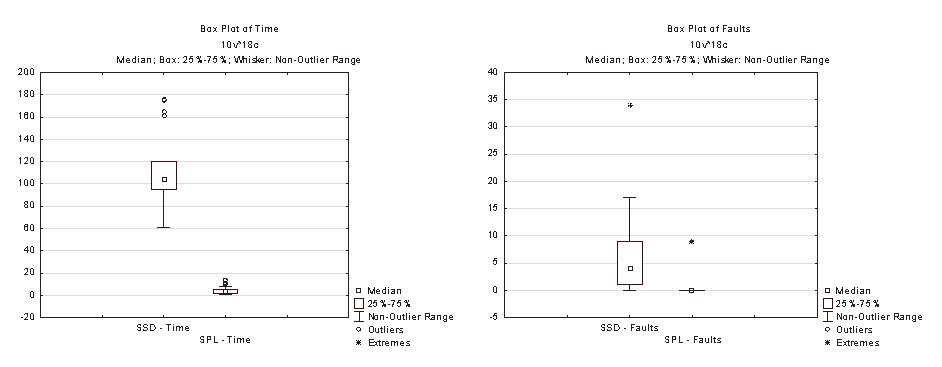
\includegraphics[scale=1.0]{./figures/section4/boxplot.eps}
\centering
\caption{Collected Data Box-Plot from SSD and SPL faults and SSD and SPL time-to-market.}
\label{fig:boxplot}
\end{figure}

\subsubsection{Hypothesis Testing}

Based on the results obtained by the use of SSD and SPL to the development of two mobile learning products, we summarize, analyze and interpret the SSD and SPL collected data (Table \ref{tab:resul1} and Figure \ref{fig:boxplot}) by means of the Shapiro-Wilk normality test and the Mann-Whitney-Wilcoxon hypothesis test. Both of them were used to validated the statistical power of the sample, allowing test the hypotheses.

\subsubsection{Efficiency in the Time of Implementation (R.Q.1)}

\begin{itemize}

\item \textbf{Collected Data Normality Tests:} the Shapiro-Wilk \cite{shaphirowilk65} normality test was applied to SSD and SPL time and faults, providing the following results:\\

\textbf{\textit{SSD time (\textit{N}=18):}}

For a mean value ($\mu$) 113.33, standard deviation value of ($\sigma$) 33.98, the time for the SSD was \textit{p} = 0.0274.

In the \textit{Shapiro-Wilk} test for a sample size \textit{(N)} 18 with 95\% of significance level ($\alpha$ = 0.05), \textit{p} = 0.0274 (0.0274 $<$ 0.05) and calculated value of \textit{W} = 0.8813 $<$ \textit{W} = 0.8970, the sample is considered non-normal.

\textbf{\textit{SPL time (\textit{N}=18):}}

For a mean value ($\mu$) 4.50, standard deviation value of ($\sigma$) 3.75, the time for the SPL was \textit{p} = 0.0014.

For a sample size \textit{(N)} 18 with 95\% of significance level ($\alpha$ = 0.05), \textit{p} = 0.0014 (0.0014 $<$ 0.05) and calculated value of \textit{W} = 0.7978 $<$ \textit{W} = 0.8970, the sample is considered non-normal.

\item \textbf{Mann-Whitney-Wilcoxon for SSD and SPL time samples:} a rank with weights were assigned for each sample value. The weights were added and applied in Equation \ref{eq:MWW}:
\small
\begin{equation}
\begin{split}
\label{eq:MWW}
U(DM) = N_1 * N_2 + \frac{N_1*(N_1+1)}{2} - \sum_{i=1}^{n} total_{2}
\end{split}
\end{equation}
\normalsize 
Where:
\begin{itemize}
\item \textit{$U(DM)$} is the equation for each of the independent sample (DM);
\item \textit{$N_1$} is the size of the sample for the X methodology that will be calculated;
\item \textit{$N_2$} is the size of the sample for the compared methodology (Y); and
\item \textit{$total_{2}$} is the sum of the weight given for the compared methodology.
\end{itemize}

For SSD the time value calculated with the Equation \ref{eq:MWW} was 326.5 and for SPL, the time value was 0.00.

Each weight matches with participant's development process time with SSD or SPL methodology. There are evidences that both values are differents ($326.5>0$), which leads to reject the null hypothesis ($H_0$) and accepted the alternative hypothesis ($H_{2}$).

Therefore, the answer for R.Q.1 was obtained: it means that the SPL is more efficient than the SSD to implement software products for mobile platform. The project base and the SPL used in the experiment need to be considered.

The participants received the base project of the two software products to be developed using SSD or SPL. The projects base consists by similarities of the products and were developed to reduce the experimental execution duration. They were implemented in 480 minutes (8 hours).

If we consider the time lasting for the implementation of each project base, plus the total of development time to each participants (480 minutes), the total time would be of 10680 minutes or 178 hours ($total_{time}$((subje\allowbreak cts(18) x minutes(480)) + 2040 = 10680 minutes). Taking into account the base project of the software product line, the time lasting by the 18 participants was 81 minutes (1 hour and 35 minutes) and the total time would be 11361 minutes or 189 hours and 35 minutes ($total_{time}$((participants(18) x minutes(4.5)) + 10599 = 11361 minutes). 

Comparing both values, the SPL development used 621 minutes (11 hours and 35 minutes) more than with SSD. However, after the SPL implementation, the line allows the evolution and insertion of new variabilities, guaranteeing the faster generation of new products in addition to other advantages of the adoption of SPL approach.

\end{itemize}

\subsubsection{Number of faults of the created software products (R.Q.2)}

\begin{itemize}

\item \textbf{Collected Data Normality Tests:} 

\textbf{\textit{SSD faults (\textit{N}=18):}}

For a mean value ($\mu$) 7.11, standard deviation value of ($\sigma$) 4, the faults for the SSD was \textit{p} = 0.0006 for the \textit{Shapiro-Wilk} normality test.

For a sample size \textit{(N)} 18 with 95\% of significance level ($\alpha$ = 0.05), \textit{p} = 0.0006 (0.0006 $<$ 0.05) and calculated value of \textit{W} = 0.7740 $<$ \textit{W} = 0.8970, the sample is considered non-normal.

\textbf{\textit{SPL faults (\textit{N}=18):}}

For a mean value ($\mu$) 1.00, standard deviation value of ($\sigma$) 0, the faults for the SPL was \textit{p} = 0.00000007 for the \textit{Shapiro-Wilk} normality test.

For a sample size \textit{(N)} 18 with 95\% of significance level ($\alpha$ = 0.05), \textit{p} = 0.00000007 (0.00000007 $<$ 0.05) and calculated value of \textit{W} = 0.3730 $<$ \textit{W} = 0.8970, the sample is considered non-normal.

\item \textbf{Mann-Whitney-Wilcoxon for SSD and SPL faults samples:} for SSD the number of faults calculated with the Equation \ref{eq:MWW} was 282 and for SPL, the number of faults was 42.

Each weight matches with participants development project faults with SSD or SPL methodology. There are evidences that both values are differents ($282>42$), which leads to reject the null hypothesis ($H_0$) and accepted the alternative hypothesis ($H_{1}$).

Therefore, based on the result from the Mann-Whitney-Wilcoxon, the answer for R.Q.2 was obtained: it means that the SSD is prone to showed more faults in the software products developed than the SPL.

\end{itemize}

\subsection{Interpretation and Discussion}\label{sub:interpretation}

Data collected from SSD and SPL application was analyzed and interpreted. Results are summarized in Table \ref{tab:resul_s}.

\begin{table}[!ht]
\caption{\label{tab:resul_s}SSD and SPL Normality and Statistical Tests Results.}
\centering
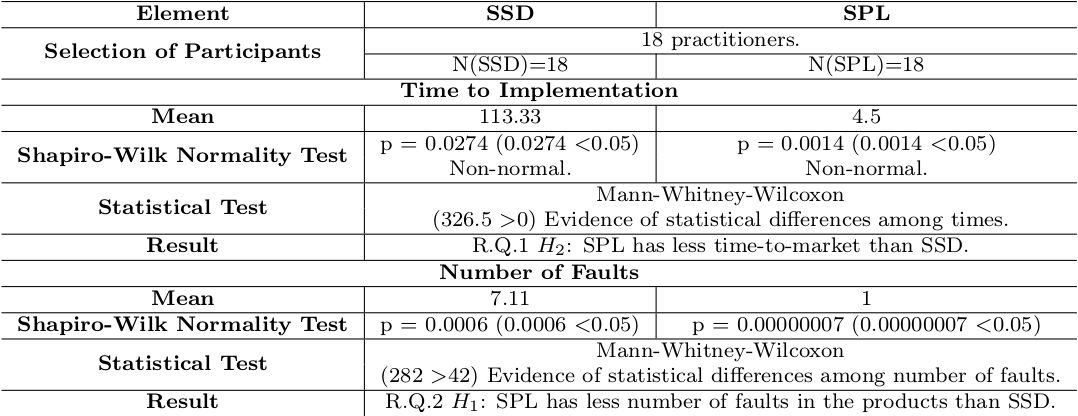
\includegraphics[scale=0.360]{figures/section4/MSPLExpSummary.png}

%\scriptsize
%\resizebox{0.87\textwidth}{!}{\begin{minipage}{\textwidth}
%\begin{tabular}{ccc}
%\hline
%\multicolumn{1}{c|}{\textbf{Element}}                                      & \multicolumn{1}{c|}{\textbf{SSD}}                          & \textbf{SPL}                                 \\ \hline
%\multicolumn{1}{c|}{\multirow{2}{*}{\textbf{Selection of Participants}}}       & \multicolumn{2}{c}{18 practitioners.}                                                                     \\ \cline{2-3} 
%\multicolumn{1}{c|}{}                                                      & \multicolumn{1}{c|}{N(SSD)=18}                             & N(SPL)=18                                    \\ \hline
%\multicolumn{3}{c}{\textbf{Time to Implementation}}                                                                                                                                            \\ \hline
%\multicolumn{1}{c|}{\textbf{Mean}}                                         & \multicolumn{1}{c|}{113.33}                                & 4.5                                          \\ \hline 
%\multicolumn{1}{c|}{\multirow{2}{*}{\textbf{Shapiro-Wilk Normality Test}}} & \multicolumn{1}{c|}{p = 0.0274 (0.0274 \textless 0.05)}    & p = 0.0014 (0.0014 \textless 0.05)           \\
%\multicolumn{1}{c|}{}                                                      & \multicolumn{1}{c|}{Non-normal.}                           & Non-normal.                                  \\ \hline
%\multicolumn{1}{c|}{\multirow{2}{*}{\textbf{Statistical Test}}}            & \multicolumn{2}{c}{Mann-Whitney-Wilcoxon}                                                                 \\
%\multicolumn{1}{c|}{}                                                      & \multicolumn{2}{c}{(326.5 \textgreater 0) Evidence of statistical differences among times.}            \\ \hline
%\multicolumn{1}{c|}{\textbf{Result}}                                       & \multicolumn{2}{c}{R.Q.1 $H_2$: SPL has less time-to-market than SSD.}                                                      \\ \hline
%\multicolumn{3}{c}{\textbf{Number of Faults}}                                                                                                                                \\ \hline
%\multicolumn{1}{c|}{\textbf{Mean}}                                         & \multicolumn{1}{c|}{7.11}                                  & 1                                            \\ \hline
%\multicolumn{1}{c|}{\textbf{Shapiro-Wilk Normality Test}}                  & \multicolumn{1}{c|}{p = 0.0006 (0.0006 \textless 0.05)}    & p = 0.00000007 (0.00000007 \textless 0.05)   \\ \hline
%\multicolumn{1}{c|}{\multirow{2}{*}{\textbf{Statistical Test}}}            & \multicolumn{2}{c}{Mann-Whitney-Wilcoxon}                                                                 \\
%\multicolumn{1}{c|}{}                                                      & \multicolumn{2}{c}{(282 \textgreater 42) Evidence of statistical differences among number of faults.} \\ \hline
%\multicolumn{1}{c|}{\textbf{Result}}                                       & \multicolumn{2}{c}{R.Q.2 $H_1$: SPL has less number of faults in the products than SSD.}                                    
%\end{tabular}
%\end{minipage}}
\end{table}

In terms of time-to-market, the statistical difference showed by Mann-Whitney-Wilcoxon test provides evidence that SPL (i.e., M-SPLearning) was more efficient than SSD in the development of P1 and P2 m-learning products, thus answering R.Q.1.

With regard to the number of faults, the statistical difference showed by Mann-Whitney-Wilcoxon test provides evidence that SSD showed more faults than SPL in the development of P1 and P2 m-learning products, thus answering R.Q.2.

From the results of the Mann-Whitney-Wilcoxon test, both R.Q.1 and R.Q.2 null hypotheses can be rejected.

\subsubsection{Threats to Validity}\label{sec:threats}

This section presents the actions taken to act directly against threats of this experiment, according to the Conceptual Model of Anderlin Neto and Conte \cite{neto13}.

\textbf{Internal Validity:}

\begin{itemize}
\item \textbf{Differences among participants:} as we took participants with different experience levels, variations in the participants' skills were reduced during the training sessions. The assessments realized in the end of each day of training allowed to evaluate the level of knowledge in the content used in the experimental execution, thus guaranteeing the reduction of variations in participants' skills.

\item \textbf{Fatigue effects:} on average, the experiment lasted 180 minutes. Thus, fatigue was considered not relevant since the participants were able to leave the room for a quick break. Periods of absence were registered to be not added in the period of time registered to be analysed.

\item \textbf{Influence among participants:} the participants performed the experiment under supervision of a human observer to mitigate the possible influence of communication among them.

\item \textbf{Trainning Sessions:} the explanations in training sessions were given not only for the question, but for every participant. This action was taken to avoid possible biases, and allowed that every training member stayed abreast of the answer for all doubts.
\end{itemize}

\textbf{External Validity:}

\begin{itemize}

\item \textbf{Instrumentation:} m-learning products and other instruments were tested in the pilot project, being considered significant to analyze time-to-market and number of faults.

\item \textbf{Participants:} more experiments considering different metrics with industry practitioners must be conducted in order to identify other relevant factors related to the adoption of M-SPLearning.

\end{itemize}

\begin{itemize}

\item \textbf{Construction Validity:} independent variables were tested in the pilot project to guarantee their validity.

\item \textbf{Conclusion Validity:} since the number of participants is reduced, mainly by the number of practitioners in the industry, the sample size must be increased in prospective replications of the experiment. The results of this study is considered indicators, and not conclusive, although, the lack of experimental executions in industrial environment, even with small samples are important for the evaluation of the time-to-market and quality for both SSD and SPL.

\end{itemize}


\section{Lessons Learned}\label{section5}

During the execution of the activities documented in this paper, the authors identified some situations in which works related to the concepts involved can benefit. As lessons learned from the work conducted, we highlight:

\begin{itemize}
    \item \textbf{Domain Caracteristics:} domain analysis can be considered one of the most important activities for the creation of an SPL. Therefore, the evolution of the catalog of requirements proposed by Duarte Filho and Barbosa \cite{filho13} significantly contributed in terms of domain knowledge. Moreover, it supported the adoption of the proactive model to the development of M-SPLearning.
    \item \textbf{Variabilities and M-Learning:} the use of the SMarty notation helps to identify the variation points during the design of M-SPLearning, ensuring greater cohesion for implementing the SPL components. The notation also contributes to the assimilation of the concept of SPL. However, it is necessary to train those involved so that the elements of notation can be used consistently.
    \item \textbf{M-SPLearning Development:} it is important to notice that implementing something generic and customizable is significantly different of to implement something static. Therefore, developing features in an SPL is considerably more labor intensive, which is justified by the subsequent gains of reuse.
    \item \textbf{M-SPLearning Experimental Evaluation:} researches show that test executions in SPLs are scarce and need to be evaluated and validated \cite{engstrom11}. Thus, the authors decided to apply the tests in the products generated by the SPL, enabling the comparison with an alternative methodology of development.
  
    The experimental evaluation provided relevant results for the adoption of M-SPLearning. The choice for active participants in the industry contributed to the reduction of the training session. However, experience and understanding the concepts by the participants is always difficult to measure, even with the evaluation forms applied. 
\end{itemize}

\section{Related Work} \label{section6}

%There is a lack on literature with regard to the use of variabilities and SPL to create mobile learning applications, as it is possible to note by searching terms as ``mobile learning software product line'', ``mobile learning variabiliti'' and variations, in ACM\footnote{http://dl.acm.org/} or IEEE\footnote{http://ieeexplore.ieee.org/} search bases. Therefore, the related works has a different focus of mobile learning, although, they specify and present some open issues to be researched and explored.

Gamez et al. \cite{gamez14} proposed a self-adaptation of mobile systems with dynamic SPLs. The management of variabilities is achieved using the Common Variability Language (CVL). The authors claim that CVL allows modeling the variability separately from the base model, but both the variability and the base models appear as connected and can be managed using the same tool. %The proposal was applied in a case study and presents good results.

Marinho et al. \cite{marinho10} proposed an architecture for nested SPLs in the domain of mobile and context-aware applications. However, the authors do not specify how to improve the management of variabilities in such a domain. %The strategy used was defined a nested SPL that aims to facilitate the construction of such software by domain decompostition in two level of analysis. 

Bezerra et al. \cite{bezerra09} conducted a systematic review of SPLs applied to mobile middleware, but only six studies were significant for the review. According to the authors, the few results obtained highlight the need of more research in the area. %In the specification of techniques used to developed SPLs in to mobile middleware, standed out feature model and domain specific language.

In another systematic literature review, Chen and Babar \cite{chen11} also concluded that the status of evaluation of variability management approaches in SPL engineering was quite dissatisfactory.

Actually, there are several opportunities and open issues regarding the management of variabilities, particularly in the m-learning domain, and its formal evaluation. The need of research in the area has motivated our work.

%It is clearly visible that the related works is not directly related with our study. This few works motivated the research to analise the variabilities in the mobile learning context. The paucity of researchs presents the necessity to investigate the mainly issues and opened oportunities to explore them, such as the application of them in educational context. Other visible lack in the literature is related the experimental validation to compare the time-to-market and quality of products developed with SPL and SSD methodologies, as metioned by Chen and Muhammad \cite{chen2011systematic}.

%As can be seen, there is a need for investigating variability management in several context, research  to investigate the mainly issues and opened oportunities to explore them, such as the application of them in educational context lack of As pointed out by Chen and Muhammad \cite{chen2011systematic}. Other visible lack in the literature is related the experimental validation to compare the time-to-market and quality of products developed with SPL and SSD methodologies, as metioned by Chen and Muhammad \cite{chen2011systematic}.

%The needs to explore them and experimentally evaluation the real beneficts of this methodology it is justify, not only by the reports in software product line studies in other domains, but the possibilite of the adoption of a variability management approach and SPL paradigm as a new oportunity to replace the traditional single development.

%A incipiência de estudos experimentais no contexto de linhas de produto, que comparem este paradigma de reutilização de artefatos de software com outras metodologias de desenvolvimento é claramente visível, como menciona Chen e Muhamad em sua revisão sistemática da literatura \cite{chen2011systematic}. A escassez de trabalhos neste sentido levou a busca de trabalhos isolados de avaliação de paradigmas de desenvolvimento para a condução do presente estudo. 


\section{Conclusions and Future Work}\label{section7}

%Atualmente, de acordo com a International Telecommunication Union (ITU), a quantidade de assinaturas móveis em todo o mundo aproxima-se do número de pessoas na terra. Nesse contexto, a plataforma Android mostrou-se mais relevante no domínio das aplicações m-learning, devido a sua quantidade de usuários potenciais. Com isso, este trabalho propõe uma LPS cujo principal objetivo é proporcionar maior reúso e padronização para esse domínio de aplicações.
%Nowadays, according to the International Telecommunication Union (ITU) \cite{itu14}, the number of mobile subscriptions around the world approaches the number of people on Earth. In this context, the Android platform was more relevant in the field of m-learning applications, due to its amount of potential users. Thus, 


This work proposes a LPS whose main objective is to provide greater reuse and standardization for this domain of applications.

%For this, we discussed how the variability management can improve the development of software products, particularly in the context of m-learning applications. We described M-SPLearning, which supports the development of customizable m-learning applications according to the basics of SPLs.

%Nesse cenário, o tempo necessário para o desenvolvimento dessas aplicações é essencial para que elas cheguem mais rapidamente a seus usuários finais. Desta forma, o estudo do conceito de LPS convergiu com a necessidade em questão e resultou na concepção da M-SPLearning.
In this scenario, the time required for the development of these applications is essential for them to come more quickly to their end users. Thus, the study of the concept of SPL converged to the need in question and resulted in the conception of M-SPLearning.

To support our ideas, we experimentally evaluated the use of M-SPLearning with respect to the singular software development. The obtained results were significant for the reuse approach, showing a reduction on time-to-market and a better quality in terms of faults when considering the software products developed with the support of variabilities. 

It is also important to highlight that the SMarty approach was crucial to the development of M-SPLearning, providing cost savings and better quality to the software products developed.

%Como trabalhos futuros, pretende-se evoluir a M-SPLearning com base nos insumos fornecidos a partir de sua avaliação empírica. Nesse sentido, ainda existe uma quantidade significativa de informações que podem induzir a novas linhas de pesquisa e avaliações experimentais.
As future work, we intend to evolve M-SPLearning based on the inputs provided by the empirical evaluation performed. In this sense, there is still a significant amount of information that can lead to new research lines and experimental evaluations.

%Além disso, para que a M-SPLearning possa ser avaliada em sua totalidade, todas as features elicitadas pelo catálogo de requisitos devem ser devidamente implementadas. Desta forma, um estudo empírico envolvendo a LPS propriamente dita pode ser conduzido, porque nosso experimento aferiu apenas os produtos da M-SPLearning.
Moreover, to a whole evaluation of M-SPLearning, all features elicited by catalog requirements must be properly implemented. Therefore, an empirical study involving the LPS itself can be conducted, because our experiment measured only M-SPLearning products.

%Considerando o domínio explorado, a plataforma Android vem recebendo constantes contribuições em sua estratégia de desenvolvimento. Com isso, o aperfeiçoamento da M-SPLearning deve sempre considerar a avaliação de novas ferramentas, fazendo com que a LPS evolua de acordo com as tendências do mercado.
%Considering the explored domain, the Android platform has received ongoing contributions to its development strategy. Thus, the improvement of M-SPLearning must always consider the evaluation of new tools, causing the LPS evolve according to market trends.

%Para avaliação das evoluções da M-SPLearning novos experimentos devem ser conduzidos, explorando vertentes relevantes para contexto educacional. Nesse sentido, avaliar os produtos gerados considerando variáveis como usabilidade e efetividade devem proporcionar resultados expressivos para este estudo. Além disso, as aplicações móveis resultantes podem ser aplicadas  em cenários reais de ensino e aprendizagem, com o objetivo de avaliar a M-SPLearning aplicada ao seu domínio de usuários.
%evolutions of 
To evaluate the M-SPLearning new experiments should be conducted, exploring relevant  aspects to educational context. In this sense, evaluate the products considering variables such as usability and effectiveness should provide significant results for this study. In addition, the resulting mobile applications can be applied in real scenarios of teaching and learning, in order to evaluate the M-SPLearning applied to your potential users.

%Outra perspectiva interessante está relacionada à investigação das outras estratégias de adoção propostas por. O modelo extrativo poderia ser aplicado a produtos externos a M-SPLearning, com o objetivo de expandir suas features. Além disso, o modelo reativo poderia ser estudado como uma alternativa para evoluções futuras da LPS proposta.
We also intend to investigate the use of other adoption models \cite{krueger02}. For instance, the extractive model can be applied in similar products to those generated by M-SPLearning aiming at increasing the validity of similarities and variabilities specified. The reactive model can be investigated as an alternative to the evolution of the proposed SPL as well.

%% The Appendices part is started with the command \appendix;
%% appendix sections are then done as normal sections
%% \appendix

%% \section{}
%% \label{}

%% If you have bibdatabase file and want bibtex to generate the
%% bibitems, please use
%%
%%  \bibliographystyle{elsarticle-num} 
%%  \bibliography{<your bibdatabase>}

%% else use the following coding to input the bibitems directly in the
%% TeX file.

\begin{thebibliography}{33}

%% \bibitem{label}
%% Text of bibliographic item

\bibitem{chen11} Chen~L, Babar~MA. 2011. A systematic review of evaluation of variability management approaches in software product lines. Information and Software Technology.

\bibitem{capilla13} Capilla~R, Bosch~J, Kang~KC. 2013. Systems and Software Variability Management. Springer.

\bibitem{bockle05} B\"{o}ckle~G, van der Linden~FJ. 2005. Software product line engineering: foundations, principles and techniques. Edited by Klaus Pohl. Springer Science \& Business Media.

\bibitem{vanderlinden07} van der Linden~FJ, Schmid~K, Rommes~E. 2007. Software product lines in action: the best industrial practice in product line engineering. Springer Science \& Business Media.

\bibitem{west12} West~M, Vosloo~S. 2012. Mobile Learning for Teachers: Global Themes. UNESCO.

\bibitem{kukulska05} Kukulska-Hulme~A, Traxler~J. 2005. Mobile Learning: a Handbook for Educators and Trainers. Routledge.

\bibitem{bezerra09} Bezerra~YM, Pereira~TAB, da Silveira~GE. 2009. A Systematic Review of Software Product Lines Applied to Mobile Middleware. Information Technology: New Generations (ITNG).

\bibitem{kinshuk03} Kinshuk~SJ, Sutinen~E, Goh~T. 2003. Mobile technologies in support of distance learning. Asian Journal of Distance Education.

\bibitem{wexler08} Wexler~S, Brown~J, Metcalf~D, Rogers~D, Wagner~E. 2008. Mobile Learning: What it is, why it matters, and how to incorporate it into your learning strategy. Guild Research.

\bibitem{falvojr14a} FalvoJr~V, Duarte Filho~NF, OliveiraJr~E, Barbosa~EF. 2014. Towards the Establishment of a Software Product Line for Mobile Learning Applications. International Conference on Software Engineering and Knowledge Engineering (SEKE).

\bibitem{falvojr14b} FalvoJr~V, Duarte Filho~NF, OliveiraJr~E, Barbosa~EF. 2014. A Contribution to the Adoption of Software Product Lines in the Development of Mobile Learning Applications. Annual Frontiers In Education (FIE) Conference.

\bibitem{oliveirajr10} OliveiraJr E, Gimenes IMS, Maldonado JC. 2010. Systematic Management of Variability in UML-based Software Product Lines. Journal Universal Computer Science.

\bibitem{bosch01} Bosch~J. 2001. Software product lines: organizational alternatives. International Conference on Software Engineering.

\bibitem{marcolino13} Marcolino~A, OliveiraJr~E, Gimenes~IMS, Maldonado~JC. 2013. Towards the Effectiveness of a Variability Management Approach at Use Case Level. International Conference on Software Engineering and Knowledge Engineering (SEKE).

\bibitem{marcolino14a} Marcolino~A., OliveiraJr~E, Gimenes~IMS, Barbosa~EF. 2014. Empirically Based Evolution of a Variability Management Approach at UML Class Level. Computer Software and Applications Conference (COMPSAC).

\bibitem{marcolino14b} Marcolino~A., OliveiraJr~E, Gimenes~IMS. 2014. Variability Management in Software Product Line UML Sequence Models: Proposal and Empirical Study. Brazilian Symposium Software Engineering (SBES).

\bibitem{bera15} Bera~MHG, OliveiraJr~E, Colanzi~TE. 2015. Evidence-based SMarty Support for Variability Identification and Representation in Component Models. International Conference on Enterprise Information Systems (ICEIS).

\bibitem{filho13} Filho~NFD, Barbosa~EF. 2013. A requirements catalog for mobile learning environments. Annual ACM Symposium on Applied Computing.

\bibitem{krueger02} Krueger~C. 2002. Easing the transition to software mass customization. Software Product-Family Engineering. Springer Berlin Heidelberg.

\bibitem{kang90} Kang~KC, Cohen~SG, Hess~JA, Novak~WE, Peterson~AS. 1990. Feature-oriented domain analysis (FODA) feasibility study. Software Engineering Institute, Carnegie Mellon University.

\bibitem{llamas14} Llamas~MSR, Reith~R, Shirer~M. 2014. Android and iOS Continue to Dominate the Worldwide Smartphone Market with Android Shipments Just Shy of 800 Million in 2013. According to IDC (Online).

\bibitem{vangurp01} Van Gurp~J, Bosch~J, Svahnberg~M. 2001. On the notion of variability in software product lines. Working IEEE/IFIP Conference on Software Architecture.

\bibitem{fielding00} Fielding~RT. 2000. Architectural styles and the design of network-based software architectures. University of California.

\bibitem{marinho10} Marinho~FG, Costa~AL, Lima~FF, Neto~JBB, Rocha~L, Dantas~VLL, Andrade~RMC, Teixeira~E, Werner~C. 2010. An architecture proposal for nested software product lines in the domain of mobile and context-aware applications. Software Components, Architectures and Reuse (SBCARS).

\bibitem{nascimento11} Nascimento~AS, Rubira~CMF and Lee~J. 2011. An SPL approach for adaptive fault tolerance in SOA. International Software Product Line Conference.

\bibitem{jedlitschka07} Jedlitschka~A, Pfahl~D 2005. Reporting guidelines for controlled experiments in software engineering. In Empirical Software Engineering. IEEE Software.

\bibitem{craig02} Craig~RD, Jaskiel~SP. 2002. Systematic software testing. Artech House.

\bibitem{wohlin12} Wohlin~C, Runeson~P, Host~M, Ohlsson~MC, Regnell~B, Wesslen~A. 2012. Experimentation in software engineering. Springer Science \& Business Media.

\bibitem{shaphirowilk65} Shaphiro~SS, Wilk~MB. 1965. An analysis of variance test for normality. Biometrika.

\bibitem{neto13} Neto~AA, Conte~T. 2013. A conceptual model to address threats to validity in controlled experiments. International Conference on Evaluation and Assessment in Software Engineering. ACM.

\bibitem{engstrom11} Engstr\"{o}m~E, Runeson~P. 2011. Software product line testing -- A systematic mapping study. Information and Software Technology.

\bibitem{gamez14} Gamez~N, Fuentes~L, Troya~J. 2014. Self-adaptation of mobile systems with dynamic software product lines. IEEE Software.

\bibitem{itu14} ITU. 2014. The world in 2014: Ict facts and figures. Information and Communication Technologies (ICT).

\end{thebibliography}
\end{document}
\endinput
%%
%% End of file `elsarticle-template-num.tex'.
